% Journal:
%   Journal of Ambient Intelligence and Smart Environments (JAISE), IOS Press
%   Web Intelligence and Agent Systems: An International Journal (wias)
%   Semantic Web: Interoperability, Usability, Applicability (SW)
% Latex 2e
% Test file iosart2c.tex

%[seceqn,secfloat,secthm,crcready]

% options: wias, jaise, sw
\documentclass{iosart2c}

\usepackage[T1]{fontenc}
\usepackage{times}%
%\usepackage{natbib}
%\usepackage[dvips]{hyperref}
\usepackage{amsmath}
\usepackage{dcolumn}
%\usepackage{endnotes}
\usepackage{graphics}
\usepackage{graphicx}
\usepackage{url}
\usepackage{longtable}
\usepackage{supertabular}
%\usepackage{lscape}
\usepackage{pdflscape}
\usepackage{longtable}
\usepackage{pifont}
\newcommand{\tick}{\ding{52}}
\usepackage{rotating}
\usepackage{array}
\usepackage{tabularx}
\usepackage{lscape}
\usepackage{multirow}
\usepackage{widetext}
\usepackage{float}
\usepackage{amsmath}
\usepackage{amsthm}
\newtheorem{definition}{Definition}
\usepackage{mathtools}
\usepackage{rotating}
\usepackage{footnote}

\newcolumntype{d}[1]{D{.}{.}{#1}}

\firstpage{1} \lastpage{5} \volume{1} \pubyear{2009}

\begin{document}
\begin{frontmatter}                           % The preamble begins here.

%\pretitle{Pretitle}
\title{Data Quality Assessment Methodologies for Linked Open Data: A Systematic Review of the Literature}

%\runningtitle{Instructions for the preparation of a camera-ready paper in \LaTeX}
%\subtitle{Subtitle}

%\review{Name Surname, University, Country}{Name Surname, University, Country}{Name Surname, University, Country}

\author[A]{\fnms{Amrapali} \snm{Zaveri}},
%\thanks{Both authors contributed equally.}},
\author[B]{\fnms{Anisa} \snm{Rula}},
\author[B]{\fnms{Andrea} \snm{Maurino}},
\author[C]{\fnms{Ricardo} \snm{Pietrobon}} and
\author[A]{\fnms{Jens} \snm{Lehmann}} and
\author[A]{\fnms{S\"oren} \snm{Auer}}

\address[A]{Universit\"at Leipzig, Institut f\"ur Informatik, D-04103 Leipzig, Germany,\\
E-mail: (zaveri, lehmann, auer)@informatik.uni-leipzig.de}
\address[B]{University of Milano-Bicocca, Department of Computer Science, Systems and Communication (DISCo),\\ Innovative Techonologies for Interaction and Services (Lab), Viale Sarca 336, Milan, Italy\\
E-mail: (anisa.rula, maurino)@disco.unimib.it}
{\address[C]{Associate Professor and Vice Chair of Surgery, Duke University, Durham, NC, USA.,\\
E-mail: rpietro@duke.edu}}

\begin{abstract}
%200 words

\end{abstract}

\begin{keyword}
data quality\sep assessment\sep survey \sep Linked Data \sep systematic review 
\end{keyword}

\end{frontmatter}

\section{Introduction}
\label{sec:intro}
The advent of semantic web technologies, as a enabler of Linked Open Data (LOD), has swept the world with an unprecedented data volume with close to 50 billion facts represented as triples.  
Although accumulating massive amounts of data is certainly a step in the right direction, data is only as good as it's quality.  
On the Data Web we have very varying quality of information and from various domains.
Biological and health care data are no exception, with widespread availability of data in a wealth of areas including drugs, clinical trials, medicine, proteins, diseases all published as Linked Data amounting to 2.3 billion triples.

Data quality is commonly defined as the \textit{fitness of use} for a certain application or use case.
However, even datasets with quality problems might be useful for certain applications, as long as the quality is in the required range.
In the case of DBpedia, for example, the data quality is perfectly sufficient for enriching Web search with facts or suggestions about common sense information, such as entertainment topics (similarly to Google's recently launched knowledge graph).
In such a scenario, where the DBpedia background knowledge can be, for example, used to show the movies Franka Potente was starring in and actors she played with it is rather neglectable if, in relatively few cases, a movie or an actor is missing.
For developing a medical application, on the other hand, the quality of DBpedia is probably completely insufficient. 
It is to be noted that inspite of varying quality on the traditional document-oriented Web, it is still perceived to be extremely useful by most people.
Consequently, the key challenge is to determine the quality of datasets published on the Web and make this quality information explicit.
Other than on the document Web, where information quality can be only indirectly (e.g. page rank) or vaguely defined, we can have much more concrete and measurable data quality indicators for structured information (i.e. data), such as correctness of facts, adequacy of semantic representation or degree of coverage.

There are already many methodologies and frameworks available for assessing data quality which address different aspects of this task by proposing appropriate tools.
Despite quality in LOD being an essential concept, few efforts are currently in place to standardize how quality tracking and assurance should be implemented.
Therefore, in this article we present a survey of existing approaches, that have been published for assessing the data quality of Linked Data datasets. 
We attempt to gather the most notable approaches proposed so far in the literature, present them concisely in a tabular format and group them under a classification scheme. 
In particular, we formalise the commonly used terminologies across papers related to data quality.
Additionally, a generalisation of the dimensions, criteria and indicators is presented along with an overview of the steps involved in the quality assessment. 
This is done to help researchers and implementors have a clearer view of existing work, thereby encouraging further experimentation.

%corpus, dimensions, exhaustive coverage,reproducible
%Add text from http://goo.gl/0Bdkn.
%Assuring data quality is problematic within SW applications as they operate on an unbound, dynamic set of autonomous data sources. 
%RDF publishers are prone to making errors which compromise the effectiveness of applications leveraging the resulting data. 

\section{Survey Methodology}
\label{sec:method}
This systematic review was conducted by two reviewers from different institutions following the procedures as described in \cite{kitchenham:2004, Moher:2009}. 
A systematic review can be conducted for several reasons such as (a) the summarisation and comparison, in terms of advantages and disadvantages, of various approaches in a field, (b) the identification of open problems, (c) the contribution of a joint conceptualization comprising the various approaches developed in a field, or (d) the synthesis of a new idea to cover the emphasized problems. 
This systematic review comprises of all the above mentioned reasons, in that, it summarises and compares various data quality assessment methodologies as well as identifies open problems focused on Linked Open Data.
Moreover, it contributes a conceptualization of the data quality assessment field and thereafter proposes a new method for data quality assessment for LOD.

\paragraph{Related surveys.}
In order to justify the need of conducting the systematic review, we first conducted a search for related surveys and literature reviews.
We did not come across any study focused on data quality assessment methodologies and tools for Linked Data. 
However, there is a comprehensive review \cite{Batini:2006}, which surveys 13 methodologies for assessing the data quality of datasets available on the web in structured or semi-structured formats.
% what's the difference: we focus on structured data, the Linked Data field only emerged after publishing of the survey, hence, certain crucial aspects such as ... are not covered.
%LOD vs databases (information systems)
%we looked at approaches of assessing linked data 
%he focused only on dimensions
%we introduced new dimensions, metrics
%we introduced assessment steps specifically for LOD as we didn't find a standardised methodology in the approaches we came across

\paragraph{Research question.}
The goal of this review is to analyse existing methodologies for assessing the quality of structured data, with particular interest in Linked Data.
To achieve this goal, we aim to answer the following general research question: \\

\emph{What are the existing approaches for assessing the quality of Linked Data?}\\

We can divide this general research question into further fine-grained research questions such as: 
\begin{itemize}
\item		\textit{What are the problems that each approach assesses?}
\item		\textit{Which are the quality dimensions and metrics supported by the proposed approaches?}
\item		\textit{What kind of tools are available for data quality assessment?}
\item		\textit{What are the assessment methods proposed by the different approaches?}
\end{itemize}

\paragraph{Define eligibility criteria.}
The eligibility criteria is an important element of any systematic review. 
First, each member created a set of inclusion and exclusion criteria on their own. 
Second, as a result of a discussion between both members a list of eligible criteria was obtained as follows:
\begin{itemize}
\item Inclusion criteria:
\begin{itemize}
\item Studies published in English between 2002 and 2012.
\item Studies focused on data quality assessment in Linked Data	
\item Studies focused on provenance assessment of Linked Data
\item Studies that proposed and implemented an approach for data quality assessment
\item Studies that assessed the quality of Linked Data and reported issues 
\end{itemize}
\item Exclusion criteria:
\begin{itemize}
\item Studies that were not peer reviewed or published
\item Methodologies that were published as a poster
\item Studies that were focused on data quality management
\item Studies that did not focus neither on Linked Data nor on structured data
\item Studies that did non propose any methodology or framework about the assessment of quality in Linked Data
%\item Studies that did not focus on quality assessment of Linked Data but only mentions the term
\end{itemize}
\end{itemize}

\begin{figure*}[ht]
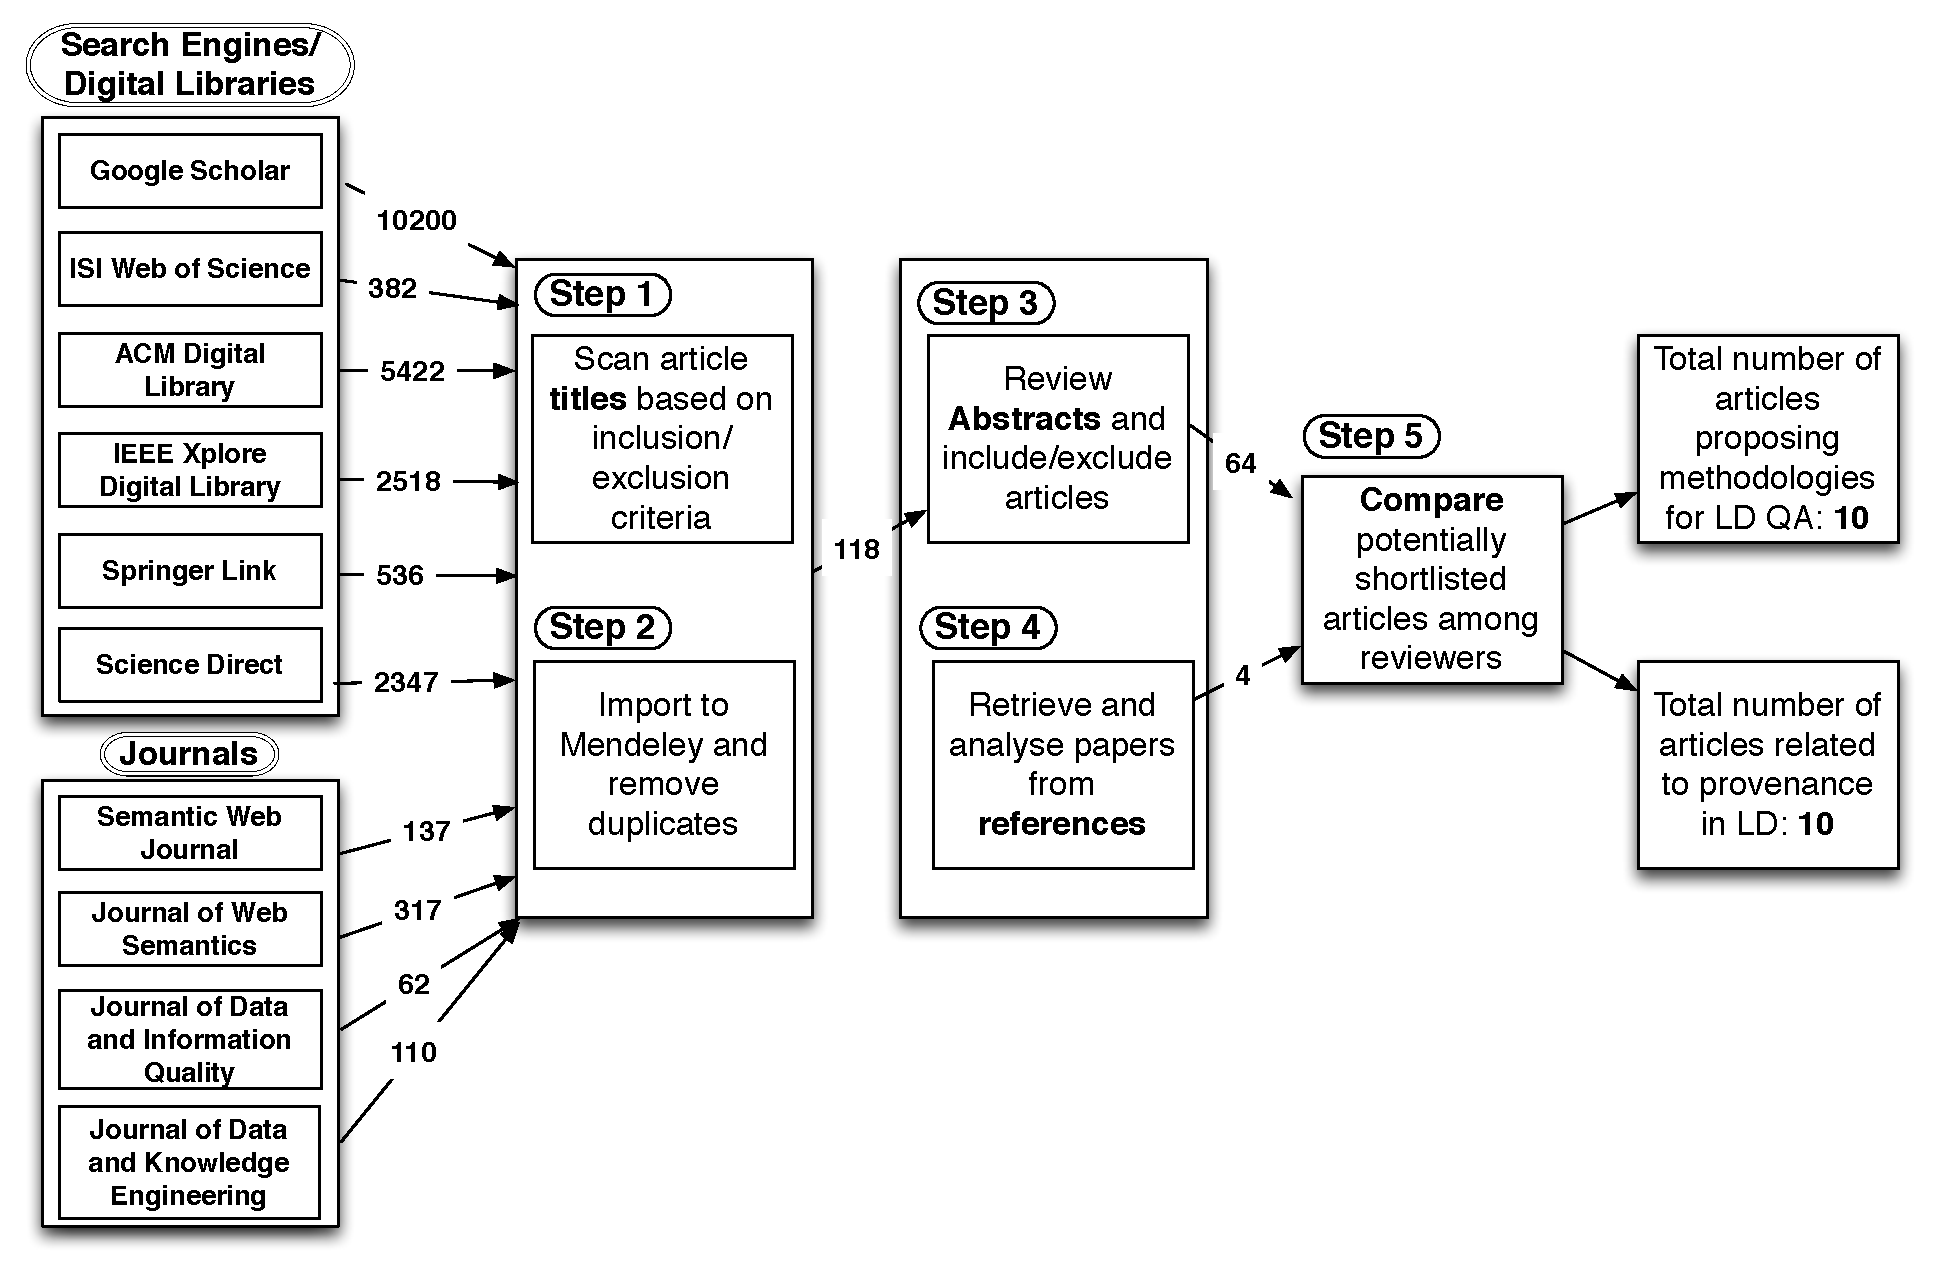
\includegraphics[width=6.5in]{Numberofarticles.pdf}
\caption{Number of articles retrieved during literature search.}
\label{fig:noofarticles}
\end{figure*}

\paragraph{Search strategy.}
Search strategies in a systematic review are usually iterative and are ran separately by both members. 
Based on the research question and the eligibility criteria, each reviewer identified several terms that were most appropriate for this systematic review, such as: \textit{data}, \textit{quality}, \textit{data quality}, \textit{assessment}, \textit{evaluation}, \textit{methodology}, \textit{improvement}, or \textit{linked data}, which were used as follows:
\begin{itemize}
\item \textit{linked data} and (\textit{quality} OR \textit{assessment} OR \textit{evaluation} OR \textit{methodology} OR \textit{improvement})
\item  \textit{data} OR \textit{quality} OR \textit{data quality} AND \textit{assessment} OR \textit{evaluation} OR \textit{methodology} OR \textit{improvement}
\end{itemize}
%The next decision was to find the suitable field (i.e. title, abstract and full-text) to apply the search
string on. 
In our experience, searching in the \textit{title} alone does not always provide us with all relevant publications. 
Thus, \textit{abstract} or \textit{full-text} of publications should also potentially be included. 
On the other hand, since the search on the full-text of studies results in many irrelevant publications, we chose to apply the search query first on the \textit{title} and \textit{abstract} of the studies.
This means a study is selected as a candidate study if its \textit{title} or \textit{abstract} contains the keywords defined in the search string.

After we defined the search strategy, we applied the keyword search in the following list of search engines, digital libraries, journals, conferences and their respective workshops: \\
Search Engines and digital libraries:
\begin{itemize}
\item Google Scholar
\item ISI Web of Science
\item ACM Digital Library
\item IEEE Xplore Digital Library
\item Springer Link
\item Science Direct
\end{itemize}
Journals:
\begin{itemize}
\item Semantic Web Journal
\item Journal of Web Semantics
\item Journal of Data and Information Quality
\item Journal of Data and Knowledge Engineering
\end{itemize}
Conferences and their Respective Workshops:
\begin{itemize}
\item International Semantic Web Conference (ISWC)
\item European Semantic Web Conference (ESWC)
\item Asian Semantic Web Conference (ASWC)
\item International World Wide Web Conference (WWW)
\item Semantic Web in Provenance Management (SWPM)
\item Consuming Linked Data (COLD)
\item Linked Data on the Web (LDOW)
\item Web Quality
\end{itemize}
Thereafter the bibliographic metadata about the 118 potentially relevant primary study were recorded using the bibliography management platform Mendeley\footnote{https://www.mendeley.com/}.

\paragraph{Titles and abstract reviewing.}
Both reviewers independently screened the titles and abstracts of the retrieved 118 articles to identify the potentially eligible articles. 
In case of disagreement while merging the lists, the problem was resolved either by mutual consensus or by creating a list of articles to go under a more detailed review. 
Then, both the reviewers compared the articles and based on mutual agreement obtained a final list of 64 articles to be included. 

\paragraph{Retrieving further potential articles.}
In order to ensure that all relevant articles were included, an additional strategy was applied such as:
\begin{itemize}
\item Looking up the reference in the selected articles
\item Looking up the article title in Google Scholar and retrieving the "Cited By" papers to check against the eligibility criteria
\item Taking each data quality dimension individually and perform a related article search
\end{itemize}
After performing these search strategies, we further retrieved 4 additional articles. 

\paragraph{Extracting data for quantitative and qualitative analysis.}
An overview of the search methodology and the number of retrieved articles at each step is shown in Figure \ref{fig:noofarticles}.
The result of the above described methodology is 21 papers from 2002 to 2012 that are reported in Table~\ref{selectedpapers} which are the core of our survey.
The next step was then to extract data from each of the articles to perform quantitative and qualitative analysis.

%\textit{To analyze the information appropriately, we required a suitable qualitative data analysis method applicable to our dataset. We used coding as our qualitative analysis methods}

\begin{table*}[htb]
\caption{List of the selected papers.} 
\label{selectedpapers}
\begin{tabular}{ | p{2.7cm} | p{10cm} | }
\hline
\textbf{Citation} & \textbf{Title} \\
\hline
Gil et.al., 2002 & Trusting Information Sources One Citizen at a Time \\
\hline
Golbeck et. al., 2003 & Trust Networks on the Semantic Web \\
\hline
Mostafavi et.al., 2004 & An ontology-based method for quality assessment of spatial data bases\\
\hline
Golbeck, 2006 & Using Trust and Provenance for Content Filtering on the Semantic Web \\
\hline
Gil et.al., 2007 & Towards content trust of web resources \\
\hline
Lei et.al., 2007 & A framework for evaluating semantic metadata \\
\hline
Hartig, 2008 & Trustworthiness of Data on the Web \\
\hline
Bizer et.al.,2009 & Quality-driven information filtering using the WIQA policy framework \\	
\hline
B\"ohm et.al., 2010 & Profiling linked open data with ProLOD \\	
\hline
Chen et.al., 2010 & Hypothesis generation and data quality assessment through association mining \\
\hline
Flemming et.al., 2010 & Assessing the quality of a Linked Data source \\
\hline
Hogan et.al., 2010 & Weaving the Pedantic Web \\
\hline
Shekarpour et.al., 2010 & Modeling and evaluation of trust with an extension in semantic web \\
\hline
F\"urber et.al., 2011 & Swiqa - a semantic web information quality assessment framework \\
\hline
Gamble et.al., 2011 & Quality, Trust, and Utility of Scientific Data on the Web: Towards a Joint Model \\
\hline
Jacobi et.al., 2011 & Rule-Based Trust Assessment on the Semantic Web \\
\hline
Bonatti et. al., 2012 & Robust and scalable linked data reasoning incorporating provenance and trust annotations \\
\hline
Gu\'eret et. al., 2012 & Assessing Linked Data Mappings Using Network Measures \\
\hline
Hogan et.al.,2012 & An empirical survey of Linked Data conformance \\
\hline
Mendes et.al.,2012 & Sieve: Linked Data Quality Assessment and Fusion \\
\hline
Rula et.al., 2012 & Capturing the Age of Linked Open Data: Towards a Dataset-independent Framework \\
\hline
\end{tabular}
\end{table*}

\paragraph{Comparison perspective of selected approaches.}
There exist several perspectives that can be used to analyze and compare the selected approaches, such as:
\begin{itemize}
\item the definitions of the core concepts
\item the dimensions and metrics proposed by each approach
\item the type of data that is considered for the assessment
\item the level of automatization of supported tools
\item the phases/steps that compose the assessment methods
\end{itemize}
Selected approaches differ in how they consider all of these perspectives and are thus compared and described in Section~\ref{concepts} and Section~\ref{sec:analysis}.

\section{Conceptualization}
\label{concepts}

There exist a number of discrepancies in the definition of many concepts in data quality due to the contextual nature of quality~\cite{Batini:2006} .
Therefore, we first describe and formally define the research context terminology (in Section~\ref{sec:general}) as well as the Linked Data quality dimensions (in Section~\ref{sec:dimensions}) in more detail.

\subsection{General terms}
\label{sec:general}
%A generalized architecture of data quality is depicted in Figure. 

\textbf{RDF Dataset.}
In this document, we understand a data source as an access point for Linked Data in the Web. 
A data source provides a dataset and it may support multiple methods of access.
The RDF triples, RDF graph and the RDF datasets have been adopted by the W3C Data Access Working Group \cite{Beckett:2004,Hayes:2004,Brickley2004}.

Given an infinite set $\mathcal{U}$ of URIs (resource identifiers), an infinite set $\mathcal{B}$ of blank nodes, and an infinite set $\mathcal{L}$ of literals, a triple $ \langle s, p, o \rangle \in (\mathcal{U} \cup \mathcal{B})\times \mathcal{U} \times (\mathcal{U} \cup \mathcal{B} \cup \mathcal{L})$ is called an RDF triple; where $s$, $p$, $o$ are the subject, the predicate and the object of the triple, respectively. An RDF graph $G$ is a set of RDF triples. A named graph is a pair  $\langle G,u \rangle$, where $G$ is called the default graph and $u\in\mathcal{U}$. An RDF dataset is a set of default and named graphs = $\lbrace G, (u_1,G_1), (u_2,G_2), ...(u_n,G_n)\rbrace$. 

\textbf{Data Quality.}
%WIQA
The concept of data quality is a domain-specific subconcept of the general concept of quality. 
A popular definition for quality is the "fitness for use"~\cite{qdefn}.
Data quality is commonly conceived as a multidimensional construct, as the "fitness for use" may depend on various factors such as accuracy, timeliness, completeness, relevancy, objectivity, believability, understandability, consistency, conciseness, availability, and verifiability~\cite{qconsumers}.

In terms of the Semantic Web, there are varying concepts of data quality.
The semantic metadata, for example, is an important concept to be considered when assessing the quality of datasets~\cite{Leigold}.
On the other hand, the notion of link quality is another important aspect in Linked Data that is introduced, where it is automatically detected whether a link is useful or not~\cite{Gueret}.
Also, it is to be noted that \textit{data} and \textit{information} are interchangeably used in the literature. 

\textbf{Data Quality Problems.}
%What is data quality problem? How the others have defined it?
The data quality problem refers to a set of issues that can affect the potentiality of the applications that use data. 
Bizer et al. \cite{Bizer} defines data quality problems as the choice of web-based information systems design which integrate information from different providers.  In \cite{Mendes} the problem of data quality is related to values being in conflict between different data sources as a consequence of the diversity of the data. 

In \cite{Flemming} the author does not provide a definition of it but implicitly explains the problems in terms of \textit{data diversity}. 
In \cite{Hogan} the authors discuss about \textit{errors} or \textit{noise} or \textit{difficulties} and in \cite{Hogan:2012} the author discuss about \textit{modelling issues} which are prone of the non exploitations of those data from the applications.
%
%%because it may be incomplete, poorly formatted, inconsistent,
%%What kind of problems we could have?
%%Errors which compromise the effectiveness of applications leveraging the resulting data. 
%%- Publishing errors; Incomplete; Incoherent; Poorly formatted; Inconsistent; Hijack; Dereferancability; Syntax errors; Link quality; Outdated; Incorrectness; Serialization problems; Inusability; System Problems; Inaccurate; Misleading; Outdated\\
%
%%Semantic Metadata
%%Data sources my have low quality such as misspelling, erroneous statements, etc; problems could be derived from the heterogeneity of data sources such as inconsistencies and duplicated entries; or be introduces by the tools employed. Changes to the data sources or to the underlying ontologies could also bring problems. 
%%data are modelled in a manner that is not
%%facilitative to generic consumption
%

\textbf{Data Quality Dimensions and Metrics.}
Data quality assessment involves the measurement of quality \textit{dimensions} or \textit{criteria} that are relevant to the consumer.
A data quality assessment \textit{metric} or \textit{measure} is a procedure for measuring an information quality dimension~\cite{Bizer}. 
These metrics are heuristics that are designed to fit a specific assessment situation~\cite{metric}.
Since the dimensions are rather abstract concepts, the assessment metrics rely on quality \textit{indicators} that allow for the assessment of the quality of a data source w.r.t the criteria~\cite{Flemming}.
An assessment score is computed from these indicators using a scoring function. 

In \cite{Bizer}, the data quality dimensions are classified into three categories according to the type of information that is used as quality indicator: (1) Content Based - information content itself; (2) Context Based - information about the context in which information was claimed; (3) Rating Based - based on the ratings about the data itself or the information provider. 

However, we identify further dimensions (defined in Section~\ref{sec:dimensions}) and also further categories to classify the dimensions, namely (1) Contextual (2) Provenance (3) Intrinsic (4) Accessibility (5) Representation and (6) Dataset Dynamicity, as depicted in Figure~\ref{fig:dimrel}.

\textbf{Data Quality Assessment Method.}
%WIQA
A data quality assessment methodology is defined as the process of evaluation if a piece of data meets in the information consumers need in a specific use case~\cite{Bizer}.
The process involves measuring the quality dimensions that are relevant to the user and comparing the assessment results with the users quality requirements.
%The steps involved in data quality assessment are: (1) formulating a research question; (2) selecting datasets and performing analyses; (3) detecting quality problems; (4) performing data quality analysis; (5) improving data quality and identifying short comings.
%%Semantic Metadata
%%There are three major steps involved in the evaluation procedure, including: setting up the evaluation context, detecting quality problems and calculating and analyzing the quality status. 

\begin{figure}
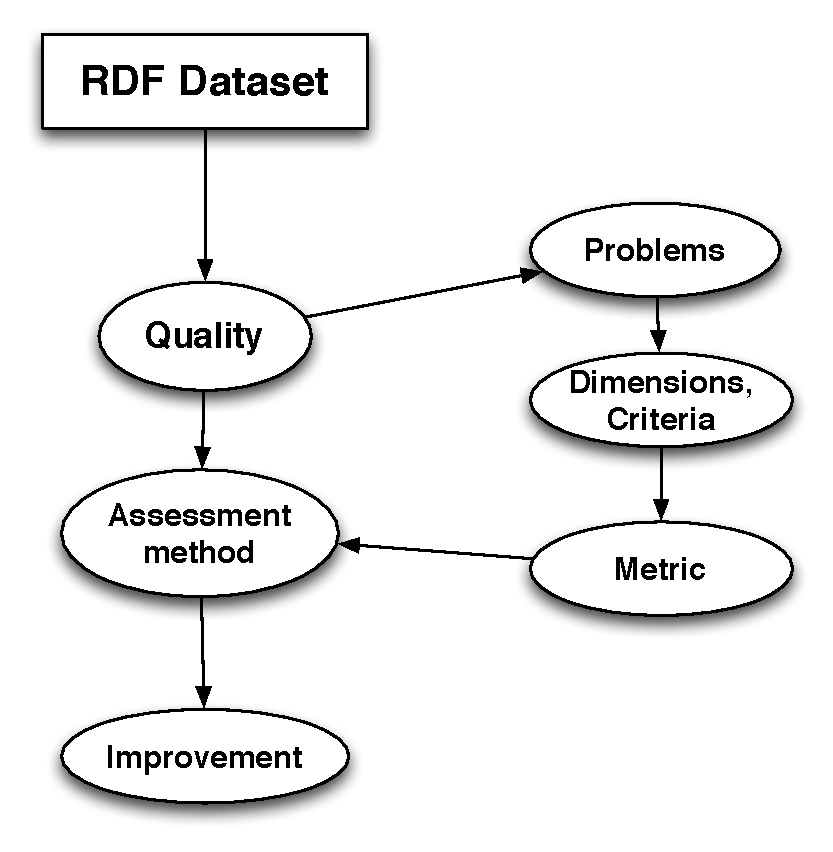
\includegraphics[scale=0.5]{Mindmap.pdf}
\caption{Conceptualization of the data quality domain.}
\label{fig:mindmap}
\end{figure}

\subsection{Linked Data quality dimensions}
\label{sec:dimensions}
% prior definitions
% our definition
%* example
%* relation to other quality dimensions
% Introduce and explain the 6 super classes of the dimensions: intrinsic, contextual, provenance, accessibility, representation, dataset dynamicity
After analyzing the 20 selected approaches, we identified 25 different data quality dimensions that can be applied to assess the quality of Linked Data. 
In this section, we formalize and adapt the definitions for each of the dimensions applicable in the Linked Data context.
Additionally, we also classify the dimensions into six different overarching groups, namely
\begin{itemize}
\item \textit{Contextual dimensions} are highly dependent on task context as well as the subjective preferences of the data consumer. %would be good to add an example to put this in context. same for the ones below
\item \textit{Provenance} focuses on the traceability and trustworthiness of the data.
\item \textit{Intrinsic dimensions} are are independent of the user's context. 
These dimensions focus on whether information correctly represents the world and whether
information maintains an internal logical consistency. 
\item \textit{Accessibility dimensions} relates to the ability to reach the data. %I would keep a distinction between data and information, these are two very different things. data is meaningless without modeling, information is what you extract out of the data 
\item \textit{Representational} dimensions capture aspects related to the design of the data such as conciseness, consistency, and data interpretability. 
\item \textit{Dataset dynamicity} relates to the timeliness of the data. 
In particular, it focuses on two aspects: the currency (if the data is up-to-date) and volatility (time period of validity) of the data.
\end{itemize}

Figure~\ref{fig:dimrel} shows the dimension classification in the above mentioned groups as well as the inter and intra relations between them.

\subsubsection{Provenance}
The ability to track the origin of data is a key component in building trustworthy, reliable applications.
%http://linkeddatabook.com/editions/1.0/#htoc47

\subsubsection{Consistency} 
Consistency implies that \emph{two or more values do not conflict with each other}~\cite{Bizerthesis}. 
Similarly Flemming et al.~\cite{Flemming} and Hogan et al.~\cite{Hogan} define consistency as \emph{when there is no contradictions in the data}. 
Mendes~\cite{Mendes} gives a more generic definition by determining a consistent dataset if it is free of conflicting information.
Consistency is considered a sub-dimension of representational consistency and is marked as an intrinsic dimension. 

An example of inconsistency is the usage of disjoint classes \cite{Hogan}: the classes \texttt{foaf:Person} and \texttt{foaf:Document} are defined as being disjoint therefore an instance cannot belong to both classes. 
%Other consistency issues identified are: improper use of inverse-functional properties, lacking usage of homogeneous datatypes, inconsistent use of terms in a vocabulary. 

% i think these examples are absolutely essential, as they will provide context to the classification. i think that examples are so crucial that you might consider keeping a companion web site with a collection of examples, with forums where people can discuss them. examples are so crucial in the context of a classification because they will increase observer agreement, meaning that two people looking at the same data quality issue will classify it the same way
Lei et al. \cite{Lei} also determine the issue of inconsistent use of terms in a vocabulary as a problem of deficiency, which denotes the situation of an inconsistent instance defined in an ontology. 
For example, an organization ontology may define that there should be only one director for an organization. 
The inconsistency problem occurs when there are two directors in the dataset.
In \cite{Mendes} an example of inconsistency is given with the value of the total population of a city in two resources of DBpedia from two languages, namely the English and Portuguese language editions. 
If both resources contain different values for the population, in the process of integration of the dataset, this will lead to the problem of inconsistency of the value. 
% Internal consistency: Do the populations of your counties add up to the populations of your states? Do the substitutes going into your soccer matches balance the substitutes going out?

\begin{definition}[Consistency]
Consistency is always related to techniques for identifying contradictions.
Depending on the available techniques, the assessment of consistency can vary.
On the Linked Data Web semantic knowledge representation techniques are employed, which come with certain inference and reasoning strategies for revealing implicit knowledge, which then might render a contradiction.
Hence, our definition of consistency is relative to a particular logic (set of inference rules) for identifying contradictions.
\end{definition}

A consequence of our definition of consistency is that a dataset can be consistent wrt. the RDF inference rules, but inconsistent when taking the OWL2-QL reasoning profile into account.
For assessing consistency, we can employ an inference engine or reasoner, which supports the respective expressivity of the underlying knowledge representation formalism.
In practice, RDF-Schema inference and reasoning with regard to the different OWL profiles can be used.
For domain specific applications, consistency rules can be defined, for example, according to the SWRL~\cite{Horrocks} or RIF standards~\cite{Kifer} and processed using a rule engine.

\subsubsection{Timeliness}
An important aspect of data is their update over time. The main time-related dimension proposed in the literature is timeliness. However, there are two more dimensions related to time aspect such as currency and volatility.
Timeliness is defined as the degree to which information is up-to-date \cite{Bizerthesis} while in \cite{Flemming} the authors defines timeliness criterion as the currentness of the data provided by a source. The definition given in Mendes et al. corresponds to the distance between the input date from the provenance graph to the current date. The recent data receives scores closer to 1 \cite{Mendes}. Similarly Rula et al. describes currency defined as the age of data given as a difference between the current date and the date when the information is last modified in the system and provides two types of currency based on document and graph level \cite{Rula2012}.
\begin{definition}[Timeliness]
Timeliness is related to measurements of data freshness. Measuring timeliness, requires available temporal meta-information attached with data which can employ different representation approach. On the Linked Data Web, the approach employed can be metadata-based representation such as Dublin Core,  reification-based representation or n-ary based representation. Hence, our definition of timeliness is relative to a particular set of temporal information, which are represented based on one of the above approaches, for measuring the distance between the current value and the last modified value of the data. 
\end{definition}

\subsubsection{Accuracy}
Bizer et al. defined accuracy as the \emph{degree of correctness and precision with which information in an information system represents states of the real world} \cite{Bizerthesis}. 
Accuracy is an intrinsic dimension i.e. it is independent of the user's context. 
We found no formal definition of accuracy in any of the other articles.

However, Lei et al. describe inaccurate annotation such as \textit{inaccurate labeling} and \textit{inaccurate classification} \cite{Lei} as an example of inaccuracy. 
Inaccurate labeling is when the mapping from the instance to the object is correct but is not properly labeled. For example, the person instance Trevor Collins might be correctly identified but wrongly marked as Both Trevor Collins. 
Inaccurate classification is when the knowledge of the source object has been correctly identified but not accurately classified. 
For example, the person Enrico Motta is classified as an instance of the high level class Person rather than the more precise class Professor. 
An additional problem identified is spurious annotation where there is no object to be mapped back to for an instance. 

Based on the definition by \cite{Bizerthesis}, we identified the problem of detecting poor attributes described in B\"ohm as an example of inaccuracy.
Poor attributed are those that do not contain useful values for data entries \cite{Bohm}. 

\subsubsection{Completeness}
Bizer defines completeness as the degree to which information is not missing. Schema completeness which is the degree to which entities and attributes are not missing in a schema; column completeness which is a function of the missing values in a column; and population completeness which refers to the ratio of entities represented in an information system to the complete population \cite{Bizerthesis}. 
In other works completeness is not properly defined but introduce problems related to it and the approach of how to identify if there is a problem. Therefore, in \cite{Hogan} completeness is defined as a problem of  incompleteness which includes equatable to a dead-link in the current HTML web, a software agent will not be able to retrieve data relevant to a particular task \cite{Hogan}. In \cite{Mendes} define completeness on the schema level and the data level. On the schema level, a dataset is complete if it contains all of the attributes needed for a given task. On the data(instance) level, a dataset is complete if it contains all of the necessary objects for a given task. 

\subsubsection{Amount of data}
Amount of Data is defined as the extent to which the volume of data is appropriate
for the task at hand \cite{Bizerthesis}.
An alternative definition says that the amount of data provided by a data source influences its usability \cite{Flemming} and is appropriate to approximate a true scenario precisely without getting false negative 	\cite{Chen}. It can be observed that there is a substantial agreement on the abstract definition of the amount of data. Although a main advantage of the Web of Data compared to the traditional web is the possibility to aggregate data from several sources, the necessity to match the underlying vocabularies puts that advantage into perspective. 

\subsubsection{Availability}
Availability is defined as the extent to which information is available, or easily and quickly retrievable  \cite{Bizerthesis} and refers to the proper functioning of all access methods \cite{Flemming}. 

\subsubsection{Understandibility}
Understandability is defined as the extent to which data is easily comprehended by the information consumer \cite{Bizerthesis}. Similarly Flemming relates understandibility to the comprehensibility of data i.e. the ease with which human consumers can understand and utilize the data \cite{Flemming}.

\subsubsection{Relevancy}
Relevancy is defined as the extent to which information is applicable and helpful for the task at hand  \cite{Bizerthesis}. 

\subsubsection{Reputation}
Since there is no definition for reputation we provide one which applies in the Web of Data. Reputation can be associated with a data publisher, a person, organisation, group of people, community of practice.
The data publisher should be identifiable for a certain (part of a) dataset. Reputation is usually a score, for example, a real value between 0 and 1. There are different possibilities to determine reputation and can be classified into direct/indirect approaches. Direct - survey in a community questioned about other members.
Indirect - use links/references/page rank.
\subsubsection{Verifiability}
Verifiability is defined as the degree and ease with which the information can be checked for correctness  \cite{Bizerthesis}. Similarly Flemming refers to verifiability criterion as to the means a consumer is provided with, which can be used to examine the data for correctness. Without such means, the only way of having a certain assurance of the correctness of the data is the consumer's trust in the source  \cite{Flemming}. 

\subsubsection{Interpretability}
Interpretability is defined as the extent to which information is in appropriate languages, symbols, and units, and the definitions are clear \cite{Bizerthesis}. Issues related to meaning (part of semantic), e.g. currency in dollars.  %and in jens 

\subsubsection{Representational Conciseness}
In \cite{Bizerthesis}, representational conciseness is defined as \emph{the extent to which information is compactly represented.} 
This dimension is related to the format or Representation of the data.
%Bizer mentions that XHTML, XML and RDF do not emphasise conciseness but are rather verbose in order to be self-descriptive and unambiguous.
%Is the logical structure of the data properly represented? 

For example, in \cite{Hogan:2012}, the use of very long URIs or those that contain query parameters is an issue related to the representational conciseness. 
Keeping URIs short and human readable is highly recommended for large scale and/or frequent processing of RDF data as well as for efficient indexing and serialisation. 

\begin{definition}[Representational Conciseness]
Representational conciseness refers to the representation of the data which is compact and well formatted on the one hand but also clear and complete on the other hand. 
It can be also seen as the degree to which the structure of the available data corresponds to the data itself, rather than being too verbose. 
\end{definition}

Representation of RDF data in N3 format is considered to be more compact than RDF/XML~\cite{Flemming}.
The concise representation not only contributes to the human readability of the data but also influences the performance of data when queried. 
%However, even though with the use of abbreviations, the data is compactly represented but it affects the clarity. 

\subsubsection{Representational Consistency}
In \cite{Bizerthesis}, representational consistency is defined as \emph{the extent to which information is represented in the same format.}
This dimension is related to the format or Representation of the data.

As stated in \cite{Hogan:2012}, the re-use of well-known terms to describe resources in a uniform manner increases the interoperability of data published in this manner and contributes towards representational consistency of the dataset.
In practice, for instance, when a data provider needs to describe information about people, FOAF~\footnote{\url{http://xmlns.com/foaf/spec/}} should be the vocabulary of choice.

\begin{definition}[Representational Consistency]
Representational consistency is the degree to which the format and structure of the information conforms to previously returned information. 
Since Linked Data involves aggregation of data from multiple sources, we extend this definition to not only imply compatibility with previous data but also with data from other sources. 
\end{definition}

Re-use of well known vocabularies, rather than inventing new ones,  not only ensures that the data is consistently represented in different datasets but also supports data integration and management tasks. 
Moreover, it maximises the probability that data can be consumed by applications that may be tuned to well-known vocabularies, without requiring further pre-processing of the data or modification of the application.
Even though there is no central repository of existing vocabularies, suitable terms can be found in SchemaWeb~\footnote{\url{http://www.schemaweb.info/}}, SchemaCache~\footnote{\url{http://schemacache.com/}} and Swoogle~\footnote{\url{http://swoogle.umbc.edu/}}.

\subsubsection{Licensing}
\emph{In order to enable information consumers to use the data under clear legal terms, each RDF document should contain a license under which the content can be (re-)used}~\cite{Hogan:2012, Flemming}.
Additionally, the existence of a machine-readable indication (by including it in a voiD description) as well as a human-readable indication of a licence is also important.
Licensing is part of the meta-information and Provenance of a dataset.

An empirical analysis done in \cite{Hogan:2012} showed that 27 PLDs (Pay Level Domains) i.e. 14.4\% returned some licensing information for some local document.
They found that, on average, providers gave licensing information for 3.4\% of local documents.
They also identified the need for an agreed-upon licensing property and an agreed set of common license URIs.

\begin{definition}[Licensing]
One of the main aims of Linked Data is to provide users the capability to aggregate data from several sources, therefore the indication of an explicit license or waiver statement is necessary for each data source.
Indication of a license grants a consumer the right to (re-)use that data along with a condition to this (re-)use.
A source can choose a licence depending on what permits it wants to issue. 
Possible permissions include the reproduction of data, the distribution of data, and the modification and redistribution of data~\cite{Miller}.
\end{definition}

Providing licensing information increases the usability of the dataset as the consumers or third parties are thus made aware of the legal rights and permissiveness under which the pertinent data are made available.
The more permissions a source grants, the more possibilities a consumer has while (re-)using the data. 
Additional triples should be added to a dataset clearly indicating the type of license or waiver. 

\subsubsection{Performance}
In \cite{Flemming}, performance is denoted as that which \emph{comprises aspects of enhancing the performance of a source as well as measuring of the actual values.} 
However, in \cite{Hogan:2012}, performance is associated with issues such as avoiding prolix RDF features such as (i) RDF reification, (ii) RDF containers and (iii) RDF collections. 
These features should be avoided as they are cumbersome to represent in triples and can prove to be expensive to support in performance or data intensive environments.
Performance is related to the Accessibility of a dataset.

For example, \cite{Hogan:2012} identifies the hosting of unstable URIs as a problem associated with the performance of agents and applications. 
The problem could occur when remote resources are removed, changed, updated or moved and the links are not updated and thus affects the performance of a dataset. 

\begin{definition}[Performance]
Performance refers to the accessibility of a dataset, that is, the more performant a data source the more efficiently a consumer can access or process the data. 
Provision of Linked Data as an RDF dump, use of hash-URIs, are means of improving the performance of a dataset. 
Additionally, high performance can be achieved through low latency and high throughput.
Latency is the amount of time in seconds from issuing the query until the first information reaches the user.
Achieving high performance should be the aim of a dataset, however large it may be. 
\end{definition}

Since Linked Data involves the aggregation of several large datasets, they should be easily and quickly retrievable.
Also, the performance should be maintained even while executing complex queries over large amounts of data. 

\subsubsection{Objectivity} 
In \cite{Bizerthesis}, objectivity is expressed as \emph{the extent to which information is unbiased, unprejudiced and impartial.}
Objectivity is an Intrinsic dimension and overlaps with the concept of Accuracy.
It is also strong related to the Verifiability dimension, that is, the more verifiable a source is, the more objective it will be.

Objectivity highly depends on the type of information. 
For example, the height of a building can be measured objectively whereas the objectivity of product descriptions require the preference of the information provider~\cite{Bizerthesis}.

\begin{definition}[Objectivity]
Objectivity refers to the bias or opinion expressed when a data publisher interprets or analyze facts.
It is therefore defined as the degree to which data is unbiased, unprejudiced and impartial. 
Objectivity, in terms of Linked Data, is a subjective dimension that focuses on how well the data publisher can express or represent the real world data as RDF such that it is unbiased, unprejudiced and impartial. 
\end{definition}

Search engines may display biased information due to either (i) occurrence of a certain keyword on a webpage indexed by a search engine to be ranked higher for searchers or (ii) paid web sites to purposefully rank their pages higher than others. 
These kinds of bias lead to error in judgement and decision making and should be avoided. 

\subsubsection{Believability}
In \cite{Bizerthesis}, believability is explained as \emph{the extent to which information is regarded as true and credible}.
Believability is a subjective dimension, is part of the Provenance of a dataset and can be seen as expected Accuracy.
It is strongly related to the Verifiability and Reputation dimensions. 

%Example

\begin{definition}[Believability]
Believability is the degree to which the information is accepted to be correct by a user.
Therefore, it can be defined as the extent to which information is regarded or accepted as true, real and credible.
It involves the trusting of information that is provided, that is, in other words deciding which information to believe.
\end{definition}

In Linked Data, believability can only be subjectively measured and highly depends on the provenance information of the dataset. 
Tim Berners-Lee proposed~\footnote{\url{http://www.w3.org/DesignIssues/UI.html}} that Web browsers should be enhanced with an "Oh, yeah?" button to support the user in assessing the reliability of data encountered on the web. 
Pressing of such a button for any piece of data or an entire dataset would contribute towards the trustworthiness, that is the believability, of the dataset. 

\subsubsection{Response Time}
In \cite{Bizerthesis}, response time is defined that which \emph{measures the delay between submission of a request by the user and reception of the response from the system.}
This dimension depends on the type and complexity of the request and is related to the Accessibility of a dataset.

\begin{definition}[Response Time]
Response Time measures the delay in seconds between submission of a query by the user and reception of the complete response from the information system.
It depends on several factors such as network traffic, sever workload, server capabilities and/or complexity of the user query, which affect the quality of query processing.
\end{definition}

Low response time hinders the usability as well as accessibility of a dataset.
Locally replicating or caching information are possible means of improving the response time.
Another option is by providing low latency, so that the user is provided with a part of the results early on.

\subsubsection{Security}
Security is a dimension which points to \emph{the possibility to restrict access to the data and to guarantee the confidentiality of the communication between a source and its consumers.} 
This dimension is related to the Accessibility of a dataset.

\begin{definition}[Security]
Security can be defined as the extent to which access to data can be restricted and hence kept secure.
It refers to the degree with which information is passed securely from users to the information source and back. 
Security covers technical aspects of the accessibility of a dataset, such as secure login and the authentication of a information source by a trusted organization.
\end{definition}

However, this dimension does not have widespread applicability in Linked Data since it mandates that the data should be open and not restricted for use, albeit with an indication of a license. 
On the other hand, adequate protection of a dataset is an important aspect to be considered against its alteration or misuse and therefore a reliable and secure infrastructure of storing a dataset is important.

\subsubsection{Uniformity}
In \cite{Flemming}, uniformity is defined as \emph{the usage of established techniques in order to increase the usability of the data.}, similar to the Representational Consistency dimension.
Uniformity is part of the Representation of a dataset as it recommends the usage of established formats and vocabularies, referencing URIs of established datasets and stating the content-types as specifically as possible.

For example, in~\cite{Hogan}, it was observed that RDF/XML content content was commonly returned with a content-type other than \texttt{application/rdf+xml}, such as \texttt{text/xml} (9.5\%) or \texttt{application/xml} (5.9\%) or \texttt{text/plain} (1\%) or \texttt{text/html} (0.4\%).

\begin{definition}[Uniformity]
The uniformity dimension refers to the usage of established techniques in order to represent data in a consistent format . 
Standardized formats such as RDF/XML, N3 or RDFa for data representation should be used to represent the data. 
Additionally, specification of a correct content-type, usage of established vocabularies and adding references of established URIs contribute towards the uniformity of the data. 
\end{definition}

The presence of uniformity in a dataset increases the usability of the data as it enables the consumer to process the data easily and also increases the chances of connecting the dataset with others.
Moreover, it helps to better understand the data as the semantics of a particular entity may be better represented using an established URI.

\subsubsection{Versatility} 
In \cite{Flemming}, versatility is referred to as the \emph{alternative representations of the data and its handling.}
Versatility is part of the Representation of a dataset.

\begin{definition}[Versatility]
Versatility mainly refers to the alternative representations of data and its subsequent handling. 
Additionally, versatility also corresponds to the provision of alternative access methods for a dataset.
Furthermore, handling of these versatile representations and access methods is an important aspect to be considered. 
Thus, versatility is defined as the alternative representations and also alternative access methods of a dataset as well as its subsequent handling. 
\end{definition}

Provision of Linked Data in different languages contributes towards the versatility of the dataset with the use of language tags for literal values.
Also, providing a SPARQL endpoint as well as an RDF dump is an indication of the versatility of the dataset.
Provision of Linked Data in the HTML format is also recommended to increase human readability.  
Similar to the Uniformity dimension, Versatility also enhances the probability of consumption and ease of processing of the data.
In order to handle the versatile representations, content negotiation should be enabled whereby a consumer can specify accepted formats and languages by adding a corresponding accept header to a HTTP request. 

\subsubsection{Validity of documents}
\emph{Validity of documents consists of two aspects influencing the usability of the documents: the valid usage of the underlying vocabularies and the valid syntax of the documents}~\cite{Flemming}. 
This is an Intrinsic dimension and related to the Accuracy, Consistency and Objectivity dimensions.

An example of the invalid usage of the underlying vocabulary is the usage of \texttt{foaf:image} instead of the defined \texttt{foaf:img}. 
Also, the use of deprecated classes and properties results in the usage of undefined terms in the future versions of these vocabularies~\cite{Hogan}. 
Another example of the invalid syntax is the assignment of improper datatypes to literals~\cite{Hogan}.
%Refer to ISWC Eval paper?

\begin{definition}[Validity of documents]
Validity of documents, in Linked Data, can be defined as the syntactic accuracy of documents, in that, it refers to not only the valid usage of the underlying vocabularies but also the valid syntax of the documents. 
Valid usage of the underlying vocabularies refers to the usage of the existing vocabularies as intended, that is, using the right semantics and in a valid context.
A syntax validator should be used to ensure the validity of RDF data, that is, the correct parsing of the triples. 
\end{definition}

RDF datasets with mistyped descriptions can result in an incorrect interpretation of the data.
Moreover, invalid usage of certain vocabularies can result in consumers not able to process data as intended.
Syntax errors, typos, not defining any additional properties that are added, use of deprecated classes and properties all add to the problem of the invalidity of the document as the data cannot neither be processedn or a consumer cannot perform reasoning on such data. 
%syntactic accuracy

\subsubsection{Conciseness}
 The authors in \cite{Mendes} characterizes conciseness as follows: \emph{On the schema level, a dataset is concise if it does not contain redundant attributes (two equivalent attributes with different names). 
Thus, intensional conciseness measures the number of unique attributes of a dataset in relation to the overall number of attributes in a target schema.
On the data (instance) level, a dataset is concise if it does not contain redundant objects (two equivalent objects with different identifiers). 
Similarly, extensional conciseness measures the number of unique objects in relation to the overall number of object representations in the dataset.}

For example, as shown in \cite{Mendes}, in the data integration task of the two editions of DBpedia (from two different languages), when the two editions contain identical URIs per object, it is an example of extensional conciseness or redundancy in the dataset.

\subsubsection{Coherence}
When an RDF triple contains URIs from different namespaces in subject and object position, this triple basically establishes a link between the entity identified by the subject (described in the source dataset using namespace A) with the entity identified by the object (described in the target dataset using namespace B). 
Through the typed RDF links data items are effectively interlinked.

\begin{definition}[Coherence]
Coherence refers to the creation and maintenance of links in a (semi-) automated way to facilitate data integration.
The interlinking refers to not only the interlinking between different datasets but also internal links within the dataset itself. 
Moreover, not only the creation of precise links but also the maintenance of these interlinks is important. 
\end{definition}

In the Web of Data, it is common to use different URIs to identify the same real-world object occurring in two different datasets. 
Therefore, it is the aim of Linked Data to link or relate these two objects in order to be unambiguous. 
For example, the disease named \emph{Tuberculosis} in one dataset is the same as the disease named \emph{TB} in another dataset. 
Therefore, it is necessary to link both the URIs to enable queries over both the datasets. 
An aspect to be considered while interlinking data is to use different URIs to identify the real-world object and the document that describes it.
For example, the creation data of a person may be different than the creation data of a document that describes this person.
The ability to distinguish the two through the use of different URIs is critical to the coherence of the Web of Data~\cite{Heath}.

%Referential correspondence: If a set of data points represents some set of real-world referents, is there one and only one point per referent? If you have 9,780 data points representing cities, but 5 of them are "Chicago", "Chicago, IL", "Metro Chicago", "Metropolitain Chicago, Illinois" and "Chicagoland", that's bad.
%9. Connectedness: If you're bringing together datasets that used to be separate, are the join points represented properly. Is the US from your country list the same as (or owl:sameAs) the US from your list of presidencies and the US from your list of world cities and their populations?

\begin{figure*}[htb]
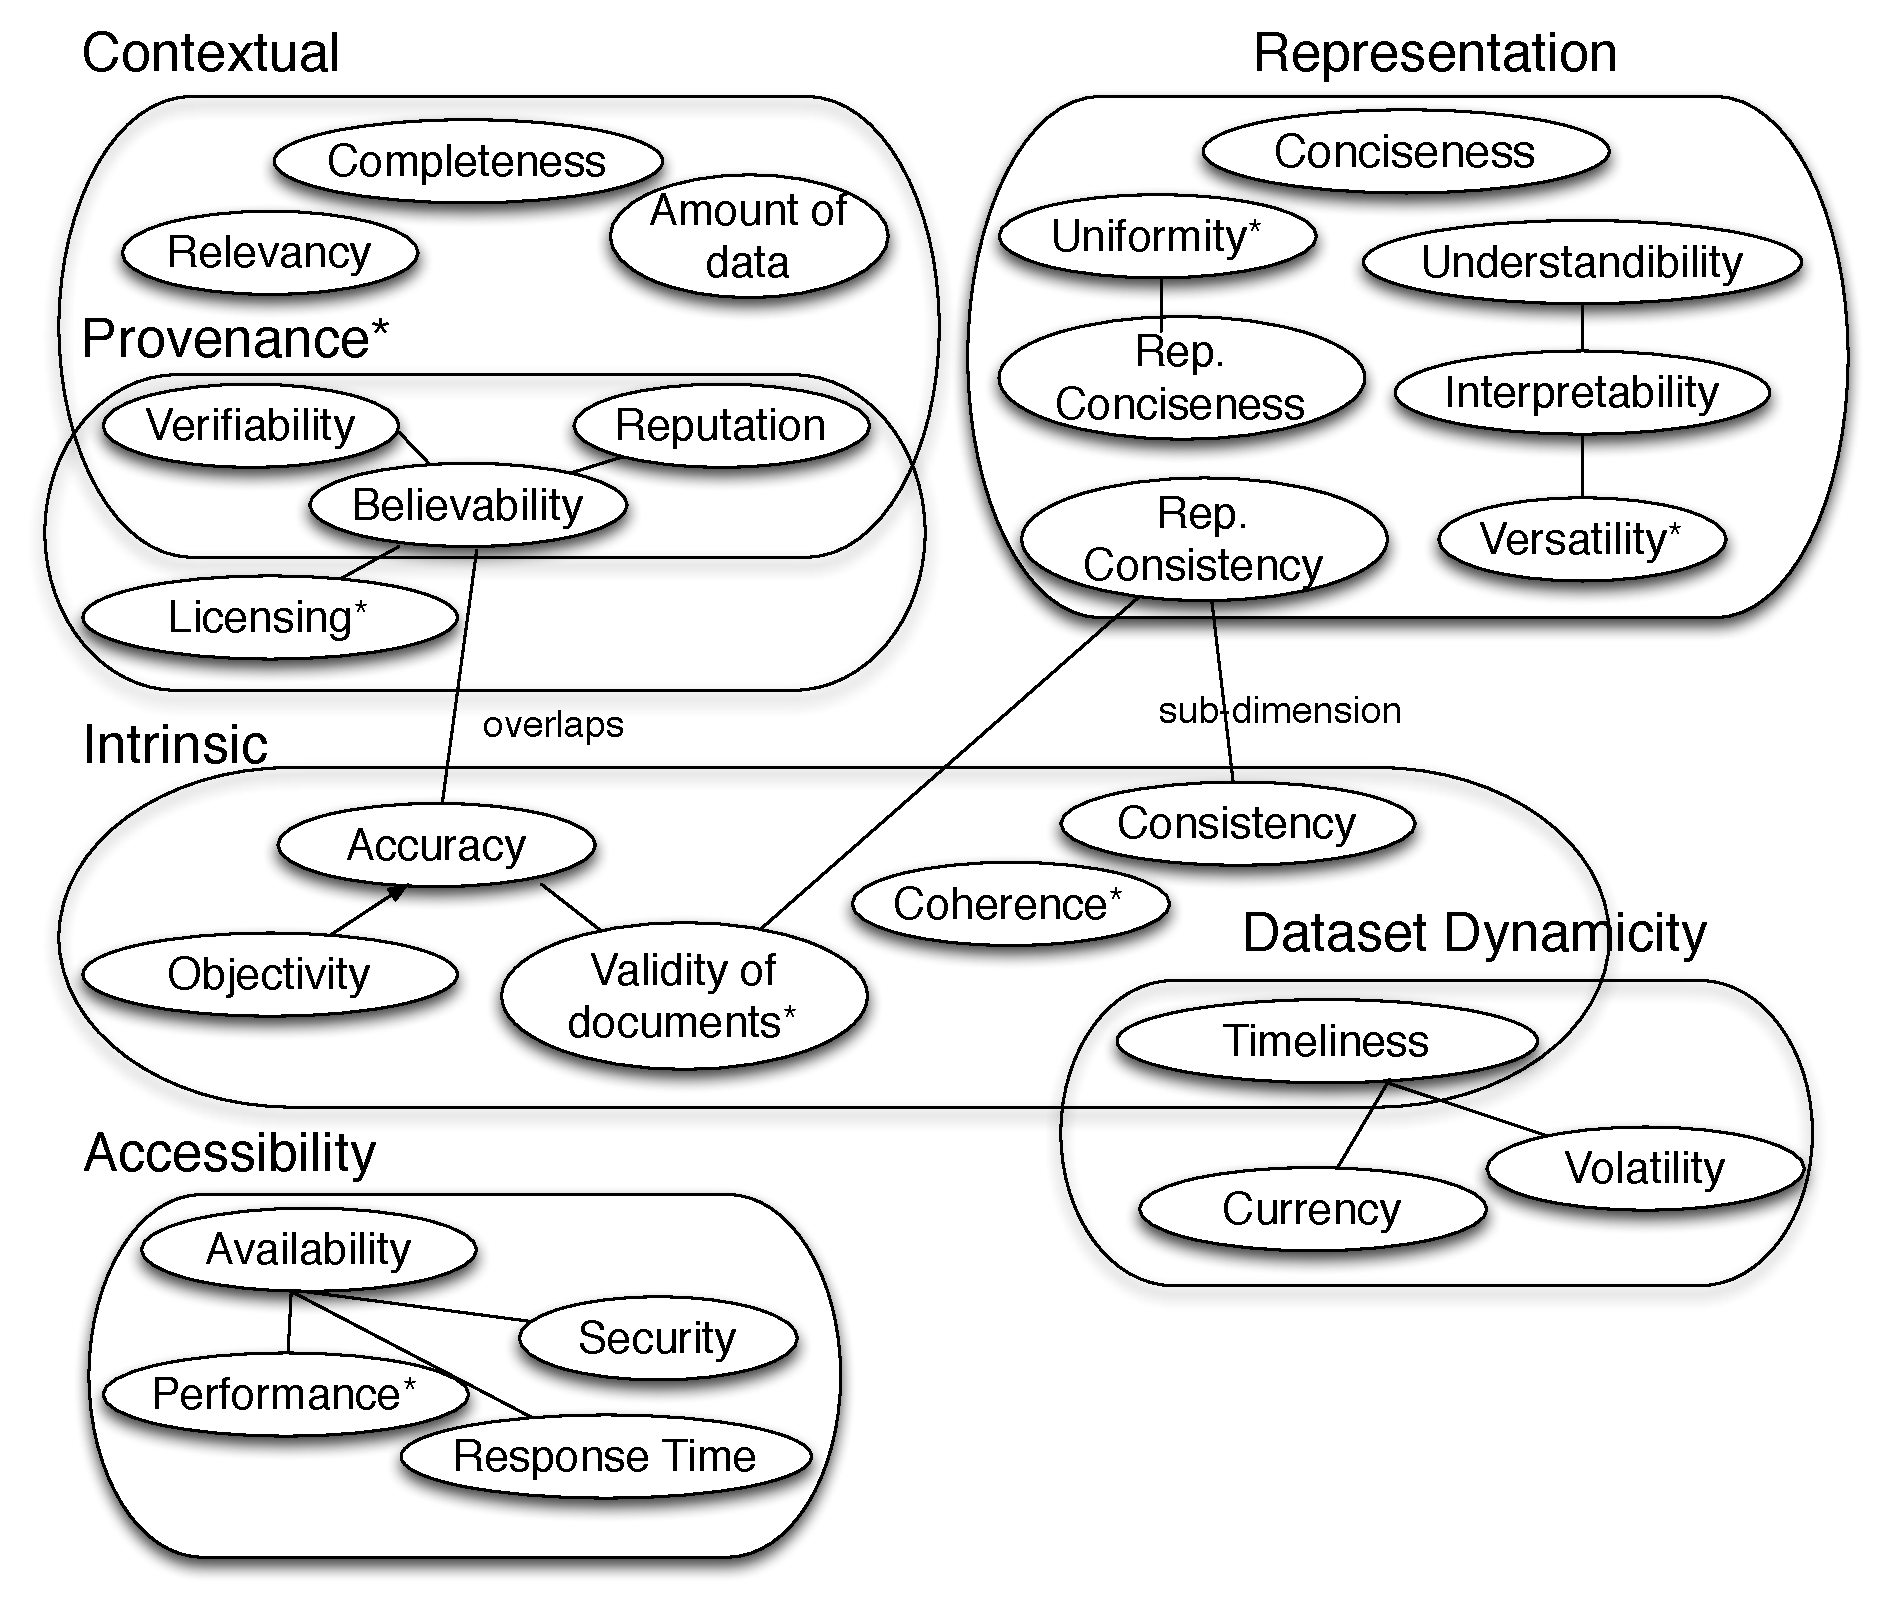
\includegraphics[width=5in]{DimensionsRelations.pdf}
\caption{Linked data quality dimensions and the relations between them.}
\label{fig:dimrel}
\end{figure*}


%\section{Results}\label{sec:results}
%This section is structured as follows:
First, we give a general overview of the results of our survey in Subsection~\ref{genoverview}.
Thereafter, we depict and discuss a conceptualisation of the data quality domain followed by a formal definition of the terminologies related to data quality in detail in Subsection~\ref{concepts}.
A quantitative evaluation of our literature review is presented in the Subsection~\ref{qntyeval} followed by a qualitative evaluation in Subsection~\ref{qltyeval}.

\subsection{General Overview}
\label{genoverview}
%Distinction between methodologies used in Linked Data and Database communities based on Open and Closed World Assumption

\subsection{Conceptualization}
\label{concepts}
\paragraph{Definition of Terminologies.}
A generalized architecture of data quality is depicted in Figure. 
There exist a number of discrepancies in the definition of many concepts, especially in data quality due to the contextual nature of quality~\cite{Batini:2006} .
Therefore, in the sequel we describe and formally define the research context terminology as well as individual components and concepts in more detail.

\textbf{RDF Dataset.}
%In this document, we understand a data source as an access point for Linked Data in the Web. It provides a dataset and it may support multiple methods of access.

The RDF triples, RDF graph and the RDF datasets have been adopted by the W3C Data Access Working Group \cite{Las99,Hayes:2004,Brickley-2004}

Given an infinite set $\mathcal{U}$ of URIs (resource identifiers), an infinite set $\mathcal{B}$ of blank nodes, and an infinite set $\mathcal{L}$ of literals, a triple $ \langle s, p, o \rangle \in (\mathcal{U} \cup \mathcal{B})\times \mathcal{U} \times (\mathcal{U} \cup \mathcal{B} \cup \mathcal{L})$ is called an RDF triple; $s$, $p$, $o$ are called, respectively, the subject, the predicate and the object of the triple. An RDF graph $G$ is a set of RDF triples. A named graph is a pair  $\langle G,u \rangle$, where $G$ is called the default graph and $u\in\mathcal{U}$. An RDF dataset is a set of default and named graphs = $\lbrace G, (u_1,G_1), (u_2,G_2), ...(u_n,G_n)\rbrace$. 

\textbf{Data Quality.}
%WIQA

The concept of data quality is a domain-specific subconcept of the general concept of quality. 
A popular definition for quality is the "fitness for use"~\cite{qdefn}.
Data quality is commonly conceived as a multidimensional construct, as the "fitness for use" may depend on various factors such as accuracy, timeliness, completeness, relevancy, objectivity, believability, understandability, consistency, conciseness, availability, and verifiability~\cite{qconsumers}.
In terms of the semantic web, there are varying concepts of data quality.
The semantic metadata, for example, is an important concept to be considered when assessing the quality of datasets~\cite{Leigold}.
On the other hand, the notion of link quality is another important aspect in Linked Data that is introduced, where it is automatically detected whether a link is useful or not~\cite{Gueret}.
Also, it is to be noted that \textit{data} and \textit{information} are interchangeably used in the literature. 

\textbf{Data Quality Problems.}
%What is data quality problem? How the others have defined it?

The data quality problem refers to a set of issues that can affect the potentiality of the applications that use data. 
In the literature there is no such a specific definition related to data quality problems. In \cite{Flemming} the author does not provide a definition of it but implicitly explains that in terms of \textit{data diversity}. In \cite{Hogan} the authors discuss about \textit{errors} or \textit{noise} or \textit{difficulties} and in \cite{Hogan:2012} the author discuss about \textit{modelling issues} which are prone of the non exploitations of those data from the applications.

Bizer et al. \cite{Bizer} defines the data quality problems as a choice of the web-based information systems design which integrate information from different providers.  In \cite{Mendes} the problem of data quality is related to values being in conflict between different data sources as as a consequence of the diversity of the data. 

%because it may be incomplete, poorly formatted, inconsistent,
%What kind of problems we could have?
%Errors which compromise the effectiveness of applications leveraging the resulting data. 
%- Publishing errors; Incomplete; Incoherent; Poorly formatted; Inconsistent; Hijack; Dereferancability; Syntax errors; Link quality; Outdated; Incorrectness; Serialization problems; Inusability; System Problems; Inaccurate; Misleading; Outdated\\

%Semantic Metadata
%Data sources my have low quality such as misspelling, erroneous statements, etc; problems could be derived from the heterogeneity of data sources such as inconsistencies and duplicated entries; or be introduces by the tools employed. Changes to the data sources or to the underlying ontologies could also bring problems. 
%data are modelled in a manner that is not
%facilitative to generic consumption

\textbf{Data Quality Criteria.}
%dimension, criteria
%indicators, metric, measures

Data quality assessment involves the measurement of quality \textit{dimensions} or \textit{criteria} that are relevant to the consumer.
A data quality assessment \textit{metric} or \textit{measure} is a procedure for measuring an information quality dimension~\cite{Bizer}. 
These metrics are heuristics that are designed to fit a specific assessment situation~\cite{metric}.
Since the criteria are rather abstract concepts, the assessment metrics rely on quality \textit{indicators} that allow for the assessment of the quality of a data source w.r.t the criteria~\cite{Flemming}.
An assessment score is computed from these indicators using a scoring function. 

The data quality assessment metrics can be classified into three categories according to the type of information that is used as quality indicator: (1) Content Based - information content itself; (2) Context Based - information about the context in which information was claimed; (3) Rating Based - based on the ratings about the data itself or the information provider~\cite{Bizer}. 

\textbf{Data Quality Assessment Method.}
%WIQA

A data quality assessment methodology is defined as the process of evaluation if a piece of data meets in the information consumers need in a specific use case~\cite{Bizer}.
The process involves measuring the quality dimensions that are relevant to the user and comparing the assessment results with the users quality requirements.
The steps involved in data quality assessment are: (1) formulating a research question; (2) selecting datasets and perf``xorming analyses; (3) detecting quality problems; (4) performing data quality analysis; (5) improving data quality and identifying short comings.
%Semantic Metadata
%There are three major steps involved in the evaluation procedure, including: setting up the evaluation context, detecting quality problems and calculating and analyzing the quality status. 

\begin{figure}
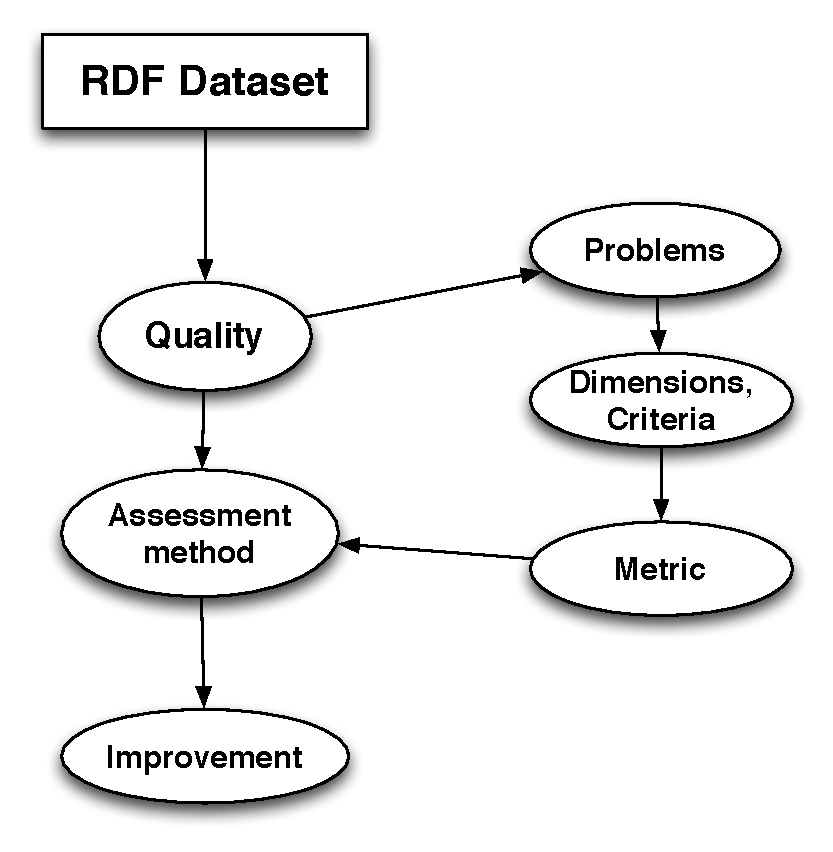
\includegraphics[scale=0.5]{Mindmap.pdf}
\caption{Conceptualization of the data quality domain.}
\label{fig:lod-life-science}
\end{figure}

\subsection{Quantitative Evaluation}
\label{qntyeval}
Out of the total number of articles retrieved from the initial literature survey, most were only related to the general aspects of data quality assessment of the data available on the Web. After refining our search strategy by using a combination of keywords and the advanced search forms available for most of the online databases, we retrieved (no.?) of articles. After reading through the articles in detail, only 9 were identified to be specifically those reporting a methodology or framework for data quality assessment of Linked Data.

%Out of the 9 articles, (no.) are from the year (?), (conference/journal).

Additionally, those articles related to provenance quality assessment, were also retrieved. A total number of (48?) articles were identified. 

\subsection{Qualtitative Evaluation}
%http://goo.gl/s2wq1
\label{qltyeval}

This section on the qualitative evaluation of the articles consists of: (i) an evaluation of each of the framework in terms of their application field, goal, target data and degree of automation of the tool, if provided; (ii) a comprehensive list of the data quality dimensions and their occurrence in the papers followed by a combination of definitions provided by several authors; (iii) a list of data quality metrics used for each of the dimensions that have been used in the papers and (iv) a generalisation of the data quality assessment steps that are followed by most authors including an account of the input and output for each step, whether a tool exists and the involvement of the user for each tool.  

\subsubsection{Qualitative evaluation of frameworks}

Table~\ref{appfield}

\begin{itemize}
\item Application field: related to whether the application covers a specific use case or covers every use case in different domains. 
\item Type of data: related to the fine grained of the data used from each paper such as triples, resources, two or more data sources and entire LOD cloud. 
\item Degree of a automation: related to the degree of interaction of the users to using the tool such as manual, semi-automated, automated. 
\end{itemize}

From the evaluation, it is observed that five out of the 20 papers focus on a very specific application or a particular domain. 
Majority of the papers develop frameworks or methodologies for the assessment of published data. 
However, most of the methodologies are only applicable at the triple or resource level. 
Six approaches, on the other hand, can be applied to two or more resources and to the entire LOD cloud.
Eight of the approaches have also implemented a tool, which is available for users to assess the quality of the LOD datasets.
The degree of automation also varies for these various tools. 
Majority of them are semi-automated or automated, two of them namely Sieve and WIQA, require a considerable amount of manual configuration and therefore requires a large amount of user involvement.  

%Then we should go into detail and describe some tool which is really useful like Flemming and Sieve and also talk about the Provenance papers in detail

\onecolumn
\begin{landscape}
\begin{table*}
\caption{Qualitative evaluation of frameworks} \label{appfield}
\begin{tabular}{ p{2.3cm} c p{7cm}  c  p{0.9cm} l p{1cm} l p{0.7cm} l cp{0.5cm} }
\hline
\textbf{Paper} & {\textbf{Application}} & \textbf{Goal} & \multicolumn{4}{c}{\textbf{Type of data}} & \multicolumn{3}{c}{\textbf{Degree of automation}} & \textbf{Tool support} \\
%\cline{2-4}
\hline
 & \textbf{G}eneral/\textbf{S}pecific &  & \textbf{Triple} & \textbf{Resource} & \textbf{Several resources} & \textbf{Entire LOD Cloud} & \textbf{Manual} & \textbf{Semi-automated} & \textbf{Automated} & \\
\hline
Bizer et.al., 2009 & G  & Information filtering & \tick & \tick & \tick & -  & \tick &  - & - & \tick \\
\hline
B\"ohm et.al., 2010 & G  & Data integration & \tick & \tick & - & - &  & \tick & -  & \tick \\
\hline
Chen et.al., 2010  & G  & Generating semantically valid hypothesis & \tick & \tick & - & - & - & - & - & - \\
\hline
Flemming et.al., 2010 & G  & Assessment of published data & \tick & \tick & - & - & - & \tick & - & \tick \\
\hline
Gu\'eret et.al., 2011 & S & Assessment of quality of links & - & - & - & \tick & - & - & \tick & \tick \\
\hline
Hogan et.al., 2010 & G &Assessment of published data by identifying RDF publishing errors and providing approaches for improvement & \tick & \tick & \tick &\tick & - & \tick & - & \tick \\
\hline
Hogan et.al., 2012 & G & Assessment of published data & \tick & \tick & \tick &\tick & - & - & - & - \\
\hline
Lei et.al., 2007 & S & Assessment of semantic metadata & \tick & \tick & - & - & - & - & - & - \\
\hline
Mendes et.al., 2012 & S & Data integration & \tick & - & - & - & \tick & - & - & \tick \\
\hline
Mostafavi et.al., 2004& S & Spatial data integration & \tick & \tick & - & - & - & - & - & - \\
\hline
Hartig, 2009 & G & Provenance model for RDF data & \tick & - & - & - & - & \tick & - & \tick \\
\hline
Hartig et.al., 2009& G & Assessment of published data using provenance information about the data on the Web to assess the quality and trustworthiness. & \tick & \tick & - & - & - & - & - & - \\
\hline
Gamble et.al., 2011& G & Application of decision networks to quality, trust
and utility assessment & - & - & \tick & \tick & - & - & - & - \\
\hline
Shekarpour et.al., 2008 & G & Method for evaluating trust & - & - & \tick & \tick & - & - & - & - \\
\hline
Golbeck et.al., 2006 & G & Algorithm for computing personalized trust recommendations using the provenance of existing trust annotations in social networks & - & - & \tick & \tick & - & - & - & - \\
\hline
Gil et.al., 2002 & G & Approach to derive an assessment of a data source
based on the annotations of many individuals & \tick & \tick & - & - & - & \tick & - & \tick \\
\hline
Golbeck et.al., 2003 & G & Trust networks on the semantic web & - & \tick & - & - & - & - & - & - \\
\hline
Gil et.al., 2007 & S & Trust assessment of web resources & - & \tick & - & - & - & - & - & - \\
\hline
Jacobi et.al., 2011 &  G & Trust assessment of web resources & - & \tick & - & - & - & - & - & - \\
\hline
Hartig et.al., 2010 & G & Trust assessment of web resources & - & \tick & - & - & - & - & - & - \\
\hline
\end{tabular}
\end{table*}
\end{landscape}
\twocolumn

\subsubsection{Data quality dimensions}

Dimensions: related to the quality dimensions identified in each work to abstractly assess data quality in LOD. 
It is possible to define a basic set of data quality dimensions, including accuracy, completeness, consistency, and timeliness, which constitute the focus of the majority of authors: 
\begin{itemize}
\item Accuracy 
%Amrapali
\item Consistency
%Anisa
\item Coherence
%Amrapali
\item Provenance
%Anisa
\end{itemize}

Table~\ref{dimex} contains a comprehensive list of the data quality dimensions and their respective definitions provided by several authors.

Table~\ref{dimensions} shows the occurrence of each dimension in the included articles. 


\begin{table*}[htb]
\caption{Data quality dimensions and their definitions.} 
\label{dimex}
\begin{tabular}{ | p{2cm} | p{12cm} | }
\hline
\textbf{Accuracy} & "the degree of correctness and precision with which information in an information system represents states of the real world." \cite{Bizer} \\
\hline
\textbf{Consistency} & "implies that two or more values do not conflict with each other." \cite{Bizer}
"The consistency criterion contains aspects indicating contradictions in the data. It can be seen a prerequisite for the correctness of the data, as inconsistent values cannot all be correct." \cite{Flemming}
"inconsistent: a software agent will interpret a contradiction in the data." \cite{Hogan}
"The deficiency identified in this category is inconsistent representation, which denotes the situation where an instance is inconsistent with the ontologies." \cite{Lei}
"A data set is consistent if it is free of conflicting information." \cite{Mendes} \\
\hline
\textbf{Objectivity} & "Objectivity is the extent to which information is unbiased, unprejudiced and impartial." \cite{Bizer} \\
\hline

\textbf{Timeliness} & "Timeliness is the degree to which information is up-to-date." \cite{Bizer}
"The timeliness criterion refers to the currentness of the data provided by a source. It is part of the correctness of the data, as outdated data might meanwhile have become invalid." \cite{Flemming}" \\
\textbf{TimeCloseness} measures the distance between the input date from the provenance graph to the current date, with more recent data receive scores closer to 1." \cite{Mendes}

In \cite{Rula}, the authors do not provide a \textit{mirefillte} definition of timeliness but they provide a definition of currency, another quality dimensions related to time, which is \textit{huazuar} from the data quality domain as "Currency is defined as a measure of the age of data" and furthermore they provide a measure of currency at document and graph level. For instance, lets consider we want to evaluate the age of the following statement: X ceoOf Y. Considering the approach we can deduce from the age of the 


\hline
\textbf{Believability} & "The extent to which information is regarded as true and credible.| \cite{Bizer} \\
\hline
\textbf{Completeness} & "Completeness is the degree to which information is not missing. Schema completeness which is the degree to which entities and attributes are not missing in a schema; column completeness which is a function of the missing values in a column; and population completeness which refers to the ratio of entities represented in an information system to the complete population." \cite{Bizer}
"incomplete: equatable to a dead-link in the current HTML web, a software agent will not be able to retrieve data relevant to a particular task." \cite{Hogan}
"On the schema level, a data set is complete if it contains all of the attributes needed for a given task. On the data(instance) level, a data set is complete if it contains all of the necessary objects for a given task." \cite{Mendes} \\
\hline
\textbf{Understandibility} & "Understandability is the extent to which data is easily comprehended by the information consumer." \cite{Bizer}
"A third criterion relating to the representation of the data is its comprehensibility, i.e. the ease with which human consumers can understand and utilize the data." \cite{Flemming} \\
\hline
\textbf{Relevancy} & Relevancy is the extent to which information is applicable and helpful for the task at hand. (Bizer) \\
\hline
\textbf{Reputation} &  \\
\hline
\textbf{Verifiability} & "Verifiability is the degree and ease with which the information can be checked for correctness." \cite{Bizer}
"The verifiability criterion refers to the means a consumer is provided with, which can beused to examine the data for correctness. Without such means, the only way of having a certain assurance of the correctness of the data is the consumer's trust in the source." \cite{Flemming} \\
\hline
\textbf{Amount of data} & "Amount of Data is the extent to which the volume of data is appropriate
for the task at hand." \cite{Bizer}
Another criterion inluencing the usability of a data source is the amount of data it provides. Although a main advantage of the Web of Data compared to the traditional web is the possibility to aggregate data from several sources, the necessity to match the underlying vocabularies puts that advantage into perspective. Thus, larger datasets should be preferred." \cite{Flemming}
"whether the amount of collected data is appropriate: If the collected data is not enough to approximate the �true� scenario precisely, we will get many wrong or coincident rules (false negative)." \cite{Chen} \\
\hline
\textbf{Rep.Consistency} & "extent to which information is compactly represented" \cite{Bizer}. "Issues related to the format (part of syntax)" \cite{} \\
\hline
\textbf{Rep.Conciseness} & is the extent to which information is in appropriate languages, symbols, and units, and the definitions are clear (Bizer). Issues related to meaning (part of semantic), e.g. currency in dollars and in jens   \\
\hline
\textbf{Availability} & "extent to which information is available, or easily and quickly retrievable." \cite{Bizer}. "refers to the proper functioning of all access methods." \cite{Flemming}\\
\hline
\textbf{Response Time} & "measures the delay between submission of a request by the user and reception of the response from the system." \cite{Bizer}. \\
\hline
\textbf{Security} &  \\
\hline
\textbf{Uniformity} & "refers to the usage of established techniques in order to increase the usability of the data." \cite{Flemming} \\
\hline
\textbf{Versatility} & "refers to alternative representations of the data and its handling." \cite{Flemming} \\
\hline
\textbf{Validity of documents} & "consists of two aspects influencing the usability of the documents: the valid usage of the underlying vocabularies and the valid syntax of the documents." \cite{Flemming} \\
\hline
\textbf{Licensing} & "without a licence, the data consumer cannot legally use the data as intended." \cite{Flemming} \\
\hline
\textbf{Performance} & "comprises aspects of enhancing the performance of a source as well as measurings of the actual values." \cite{Flemming} \\
\hline
\textbf{Conciseness} & "On the schema level, a dataset is concise if it does not contain redundant attributes (two equivalent attributes with different names). On the data (instance) level, a data set is concise if it does not contain redundant objects (two equivalent objects with different identifiers). The extensional conciseness measures the number of unique objects in relation to the overall number of object representations in the dataset." \cite{Mendes} \\
\hline
\textbf{Coherence} & \\
\hline
\textbf{Provenance} & \\
\hline
\end{tabular}
\end{table*}

\onecolumn
\begin{landscape}
%\begin{table*}[htb]
%\begin{center}
\begin{longtable}{ | p{2.3cm} | p{0.6cm} | p{0.65cm} | p{0.55cm} | p{1.27cm} | p{0.8cm} | p{0.73cm} | p{0.75cm} | p{0.55cm} | p{0.9cm} | p{1.2cm} | p{0.77cm} | p{0.7cm} | p{0.9cm} | p{1.4cm} | p{1cm} | p{0.6cm} | p{1cm} | p{0.6cm} | }
\caption{A list of data quality dimensions and their usage in each of the included papers.} 
\label{dimensions} \\
\hline
\textbf{Dimensions} & Bizer et.al., 2009 & B\"ohm et.al., 2010 & Chen et.al., 2010 & Flemming et.al., 2010 & Gu\'eret et. al, 2011& Hogan et.al., 2010 & Hogan et.al., 2012& Lei et.al., 2007& Mendes et.al., 2012 & Mostafavi et.al., 2004 & Hartig, 2009 & Hartig et.al., 2009	& Gamble et.al., 2011 & Shekarpour et.al., 2008 & Golbeck et.al., 2006 & Gil et.al., 2002 & Golbeck et. al., 2003 & Gil et.al., 2007\\
\hline
\textbf{Accuracy} & \tick & \tick & & & \tick & & & \tick & & & & & & & & & & \\
\hline
\textbf{Consistency} & \tick & \tick & \tick & \tick & & \tick & & \tick & \tick & \tick & & & & & & & & \\
\hline
\textbf{Objectivity} & \tick & & & & & & & & & & & & & & & & & \\
\hline
\textbf{Timeliness} & \tick & & & \tick & & & & \tick & \tick & & & & & & & & & \\
\hline
\textbf{Believability} & \tick & & & & & & & & & & & & & & & & & \\
\hline
\textbf{Completeness} & \tick & & & & \tick & \tick & & & \tick & & & & & & & & & \\
\hline
\textbf{Understand - ibility} & \tick & & & \tick & & & & & & & & & & & & & & \\
\hline
\textbf{Relevancy} & \tick & & & & & & \tick & & & & & & & & & & & \\
\hline
\textbf{Reputation} & \tick & & & & & & & & \tick & & & & & & & & & \\
\hline
\textbf{Verifiability} & \tick & & & \tick & & & & & & & & & & & & & & \\
\hline
\textbf{Amount of data} & \tick & & \tick & \tick & & & & & & & & & & & & & & \\
\hline
\textbf{Accuracy} & & & & & & & & & & & & & & & & & & \\
\hline
\textbf{Interpretability} & \tick & & & & & & \tick & & & & & & & & & & & \\
\hline
\textbf{Rep.Conciseness} & \tick & & & & & & \tick & & & & & & & & & & & \\
\hline
\textbf{Rep.Conssitency} & \tick & & & & & & \tick & & & & & & & & & & & \\
\hline
\textbf{Availability} & \tick & & & \tick  & & & \tick & & & & & & & & & & & \\
\hline
\textbf{Response Time} & \tick  & & & & & & & & & & & & & & & & & \\
\hline
\textbf{Security} & \tick  & & & & & & & & & & & & & & & & & \\
\hline
\textbf{Uniformity} & & & & \tick  & & & & & & & & & & & & & & \\
\hline
\textbf{Versatality}& & & & \tick  & & & & & & & & & & & & & & \\
\hline
\textbf{Validity of documents} & & & & \tick  & & & & & & & & & & & & & & \\
\hline
\textbf{Licensing} & & & & \tick & & & \tick & & & & & & & & & & & \\
\hline
\textbf{Performance} & & & & \tick & & & \tick & & & & & & & & & & & \\
\hline
\textbf{Conciseness} & & & & & & & & & \tick & & & & & & & & & \\
\hline
\textbf{Coherence} & & & & & \tick & & & & & & & & & & & & & \\
\hline
\textbf{Provenance} & & & & & & & & & & & & & & & & & & \\
\hline
%\end{tabular}
%\end{center}
%\end{table*}
\end{longtable}
\end{landscape}
\twocolumn

\subsubsection{Data quality metrics}

Metrics: related to the measurements of each work provided to assess the quality in LOD.
In general, multiple metrics can be associated with each quality dimension.
\textit{ In some cases, the metric is unique and the theoretical definition of a dimension coincides with the operational definition of the corresponding metric. 
For this reason, we make a distinction between theoretical and operational definitions of dimensions only when the literature provides multiple metrics.}
Table~\ref{metrics} provides a list of the data quality metrics for each of the dimensions, how each one can be measured and classifies it as being either subjective or objective.

\onecolumn
%\begin{table*}[htb]
\begin{longtable}{ | p{2.3cm} | p{7.5cm} | m{2cm} |  }
\caption{Comprehensive list of data quality metrics, how they can be measured and the type} 
\label{metrics} \\
\hline
\textbf{Dimension} & \textbf{Metric} & \textbf{Type of metric (Subjective/Objective)} \\
\hline
\multirow{10}{*}{Accuracy} & Interlinking & O \\
& Dereferencabiity issues & O \\
& No structured data available & O \\
& Misreported content types & O \\
& RDF/XML Sytanx errors & O \\
& Spurious annotation/representation & O \\
& Inaccurate annotation & O \\
& Inacurrate labeling and classification & O \\
& detect poor attributes & O \\
& accuracy of interlinking between datasets & O \\
\hline
\multirow{9}{*}{Consistency} & no definitions of entities as being members of disjoint classes & \\
& valid usage of inverse-functional properties & \\
& no redefinition of existing properties & \\
& usage of homogeneous datatypes & \\
& no stating of inconsistent values for properties & \\
& annotation & \\
& reasoning: noise and inconsistency & \\
& misuse of predicates & \\
& inconsistencies in ontologies & \\
\hline
Objectivitiy & no bias or opinion expressed when a data provider interprets or analyses facts & \\
\hline
\multirow{4}{*}{Timeliness} & stating the most recent validation of the data & \\
& no inclusion of outdated data & \\
& inclusion of recent data & \\
& dereferencability of all internal and external URIs & \\
\hline
\multirow{2}{*}{Believability} & meta-information about the identify of information provider & \\
& checking source from which information is retrieved & \\
\hline
\multirow{6}{*}{Completeness} & schema completeness & \\
& column completeness & \\
& population completeness & \\
& URI/HTTP: accessibility and dereferencability & \\
& linking & \\
\hline
\multirow{10}{*}{Understandibility} & human-readable labelling of classes, properties and entities by providing rdfs:label & \\
& human-readable description of classes, properties and entities by providing an rdfs:comment & \\
& indication of metadata about a dataset & \\
& indication of one or more exemplary URIs & \\
& indication of a regular expression that matches the URIs of a dataset & \\
& indication of an exemplary SPARQL query & \\
& indication of some of the vocabularies used & \\
& operability of HTML documents & \\
& provision of message boards and mailing lists & \\
& meta information about the language of web content & \\
\hline
\multirow{5}{*}{Relevancy} & using meta-information attributes & \\
& count occurrence of relevant terms within these attributes & \\
& looking for licensing meta-information like Creative Commons labels & \\
& sort documents according to their relevancy for a given query & \\
& existence of links to external data providers: use external URIs, provide owl:sameAs link & \\
\hline
\multirow{4}{*}{Verifiability} & stating basic provenance information & \\
& usage of a dedicated provenance vocabulary & \\
& usage of digital signatures & \\
& traceability and provability & \\
\hline
\multirow{4}{*}{Amount of data} & no. of triples in a dataset & \\
& no. of internal and external links & \\
& scope and level of detail - coverage & \\
& whether the amount of collected data is appropriate & \\
\hline
\multirow{5}{*}{Interpretability} & use of appropriate language, symbols, unites and clear definitions & \\
& use of self-descriptive formats, identifying objects and terms used to define the objects with globally unique identifiers & \\
& use of various schema languages to provide definitions for terms & \\
& naming resources - avoiding blank nodes & \\
& dereferenced representations - giving human readable metadata & \\
\hline
Rep. Conciseness & information is compactly represented - keep URIs short & \\
\hline
\multirow{3}{*}{Rep. Consistency} & re-use existing terms & \\
& cherry pick vocabularies & \\
& provision of data in different representational formats & \\
\hline 
\multirow{11}{*}{Availability} & accessibiliy of the server & \\
& dereferenceable URIs & \\
& host of stable URIs & \\
& URIs don't contain variable information & \\
& homogeneous (lower) case of URIs & \\
& redirection using the status code 303 See Other & \\
& accessibility of the SPARQL endpoint & \\
& accessibility of the RDF dumps & \\
& URI/HTTP: accessibility and derefencability & \\
& accessibility of the RDF dumps  & \\
& dereferenced representations:�
- dereference forward links
- dereference back-links & \\
\hline
Response time & delay between submission of a request by the user and reception of the response from the system & \\
\hline 
Security & \\
\hline
\multirow{4}{*}{Uniformity} & usage of an established format & \\
& stating the content-types as specifically as possiblet & \\
& usage of established vocabulariest & \\
& referencing of established URIst  & \\
\hline
\multirow{6}{*}{Versatility} & provision of the data in various formats & \\
& provision of the data in various languages & \\
& application of content negotiation & \\
& correct interpretation of the accept-headers sent & \\
& human-readable indication of a SPARQL-endpoint & \\
& machine-readable indication of a SPARQL-endpoint & \\
\hline
\multirow{4}{*}{Validity of documents} & no syntax errors & \\
& exclusive usage of defined classes and properties & \\
& no usage of deprecated classes and properties & \\
& usage of proper datatypes & \\
\hline
\multirow{7}{*}{Licensing} & machine-readable indication of a licence & \\
& human-readable indication of a licence & \\
& permitted reproduction of data & \\
& permitted distribution of data & \\
& permitted modification and redistribution of data & \\
& no attribution needed & \\
& no Copyleft / Share Alike needed & \\
\hline
\multirow{8}{*}{Performance} & machine-readable indication of one or more RDF dumps & \\
& human-readable indication of one or more RDF dumps & \\
& usage of Slash-URIs when providing a large amout of data & \\
& low latency & \\
& high throughput & \\
& only minor variations of the performance & \\
& maintenance of the performance no matter the load & \\
& avoid prolix RDF features & \\
\hline
\multirow{2}{*}{Conciseness} & schema level : intensional conciseness - does not contain redundant attributes & \\
& data level : extensional conciseness - does not contain redundant objects & \\
\hline
%\end{tabular}
%\end{table*}
\end{longtable}
\twocolumn

\subsubsection{Data quality assessment steps}

Table~\ref{metricsteps} comprises of the steps involved in the data quality assessment process. 

Assessment steps: related to the common steps of each work used to assess the quality in LOD. For each step we provide input and output, a supported tool and the involvement of the user in the tool usage.  
The "Assessment steps" measures the quality of data collections along relevant quality dimensions; in particular the measurement of quality dimensions is provided by a set of metrics defined for each dimension. From the selected paper we identify the following sequence of activities customized by  different data quality methods:

Requirements analysis (optional): The multidimensionality of the information quality makes it dependent on a number of factors that can be achieved by the analyses of the user requirements. The requirement analysis is optional since it is not always provided from the methods provided in LOD papers.

Data Quality Checklist: estimates only those metrics for which we may answer yes or no. 

Statistics and low-level analysis: provides some generic statistics on the dataset based on some heuristics.

Aggregated and higher level metrics: in this category we include all the metrics that are not included in the Data Quality Checklist. Furthermore, in this step the single metrics or the combination of them produce a value within a range [0;1]. 

Comparison (optional): used when the resulted measurements provided in step "Aggregated and higher level metrics" are compared to reference values such as previous values from dataset in the same domain or gold standard values, in order to enable a diagnosis of quality. 

Interpretation: gives an interpretation to the results obtained from step Data Quality Checklist or Aggregated and higher level metrics.

\begin{table*}[h]
\caption{Data quality assessment steps} 
\label{metricsteps}
\begin{tabular}{ | p{2cm} | p{3.3cm} | p{3.7cm} | p{1.5cm} | c | c | c | }
\hline
\textbf{Steps} & \textbf{Input} & \textbf{Output} & \textbf{Tool support} & \multicolumn{2}{c}{\textbf{User involvement }} & \cr
\hline
& & & & \textbf{Automated} & \textbf{Semi-automated} & \textbf{Manual} \\
\hline
\textbf{Requirements analysis (optional)} & Assessment of data quality, 2 types of users: \begin{itemize} \item who know the problem with their data \item who do not know the problem with their data \end{itemize} & - & - & - & - & - \\
\hline
\textbf{Data quality checklist} & Checklist of dimensions which have a binary evaluation & Results of the evaluation - 0 (no) or 1 (yes) & Flemming et al., 2010  & - & - & - \\
\hline
\textbf{Statistics and low level analysis} & Dataset & \multirow{3}{*}{Overview statistics of the dataset} & LODStats & \tick & - & - \\
\cline{4-7}
 & & & Google Refine & \tick & - & - \\
\hline
\textbf{Aggregated and higher level metrics} & Dimensions not included in Step 2 & \multirow{7}{3cm}{Results of the evaluation of these dimensions in a range from 0 to 1}  
 & WIQA & - & - & \tick \\
 \cline{4-7}
 & & & ProLOD & - & \tick & - \\
 \cline{4-7}
 & & & Flemming et al., 2010 & - & \tick & - \\
 \cline{4-7}
 & & & LinkQA & \tick & - & - \\
 \cline{4-7}
 & & & RDF Validator & - & \tick & - \\
 \cline{4-7}
 & & & Sieve & - & - & \tick \\
 \cline{4-7}
 & & & EvoPat & - & - & \tick \\
\hline
\textbf{Comparison (optional)} & \begin{itemize} \item Target/derived dataset \item Assessment results from step 2 and 4 \item Original dataset \end{itemize} & \begin{itemize} \item Evaluation of the representation \item Evaluation between datasets in the same domain \end{itemize} & - & - & - & - \\
\hline
\textbf{Interpretation} & Assessment results from Step 2 and 4 & Explanation of the results & WIQA & - & - & \tick \\
\hline
\end{tabular}
\end{table*}

%Butterfly effect, avalanche effect, cascading effect
%Spider Chart: http://goo.gl/rNqgD

\section{Comparison of selected approaches}
\label{sec:analysis}
In this section, we compare the selected approaches based on the different perspectives discussed in Section~\ref{sec:method}.
In particular, we analyze and compare each approach based on the dimensions (Section~\ref{sec:dim}), their respective metrics (Section~\ref{sec:met}), types of data (Section~\ref{sec:data}), level of automatization (Section~\ref{sec:auto}) and tool usability (Section~\ref{sec:tools}). 

\subsection{Dimensions}
\label{sec:dim}
%The definition of the \emph{dimensions, and metrics} to assess data quality is a critical activity. 
The linked open data paradigm is the fusion of three different research areas namely \emph{semantic web} to generate semantic connections among data sets,  \emph{world wide web} to make the data available and preferably under an open access license, and \emph{data management} for managing large quantitites of heterogeneous and distributed data.
The selected approaches use quality dimensions taken from any one of these specific areas. 
Previously published literature provides a thorough classification of data quality from a variety of dimensions.
%What kinds of classifications?  
By analyzing the multiple classifications for different quality dimensions provided by \cite{Wand:1996, Wang:1996, Redman:1997, Jarke:2010, Bovee:2003, Naumann:2002}, it is possible to distill a core of set dimensions as: accuracy, completeness, consistency and timeliness. These constitute the focus of the majority of authors Catarci et al. \cite{scannapieco:2002}.
%check citiation.
However, no general agreement on which set of dimensions defines data quality or the exact meaning of each dimension, the same problem occurring in LOD.

As mentioned in Section~\ref{concepts}, data quality assessment involves the measurement of quality dimensions that are relevant to the consumer. %is this really true?? i would guess some of them are relevant to consumers, but many are only relevant for LOD specialists
An initial list of data quality dimensions was first obtained from~\cite{Bizerthesis}.
Thereafter, each approach was analyzed to extract the problem being addressed and later mapped to one or more of the quality dimensions.
For example, the dereferenciability issues, the non-availability of structured data, and content misreportin as mentioned in~\cite{Hogan:2012} were mapped to the dimensions of Completeness as well as Availability.
However, not all the problems present in LOD could be mapped to the initial set of dimensions such as the problem of incoherency or interlinking between datasets or the problem of the alternative representations of the data and its handling i.e. the versatility of the dataset.
As a result , we obtained a further set of quality dimensions, which were particularly relevant for Linked Data.%need more details on how exactly they were derived
Table~\ref{dimensions} shows the complete list of the 25 identified Linked Data quality dimensions along with frequency and occurrence of each dimension. 

There are three visible groups (Table): (a) a set of approaches focusing only on the provenance of the datasets~\cite{Hartig2008, Gamble2011, Shekarpour2010, Golbeck2006, Gil2002, Golbeck2003, Gil2007, Jacobi2011, Bonatti2011, Rula2012}; (b) a set of approaches using more than five dimensions \cite{Bizer, Flemming, Hogan:2012, Mendes} and (c) a set of approaches focusing on very few and specific dimensions  \cite{Bohm, Chen, Gueret, Hogan, Lei, Mostafavi}.
In addition, Provenance, Consistency, Timeliness, Accuracy and Completeness are the most frequently used dimensions. 

\subsection{Metrics}
\label{sec:met}
As defined in Section~\ref{concepts}, data quality metric is a procedure for measuring an information quality dimension.
In general, multiple metrics can be associated with each quality dimension.
In some cases, the metric is unique and the theoretical definition of a dimension coincides with the operational definition of the corresponding metric. 
For this reason, we only make a distinction between theoretical and operational definitions of dimensions when the literature provides multiple metrics.

Table~\ref{metrics} provides a list of the data quality metrics for each of the dimension and classifies it as being either subjective or objective.

%Provenance
In \cite{Hartig2008} the authors determine the measurement of trustworthiness of RDF statements as a value of trust which is either unknown or a value in the [-1,1] interval. 

They do not prescribe and implementation of how to assign a trust value to the statements but instead provide a data provenance model which includes information about the publisher of the dataset, creation method and time of the dataset as well as the publisher along with publication time of possible original sources. 
Therefore the provenance information can be exploited to assess other dimensions such as timeliness or accuracy, which in turn can be merged to provide a unified value of provenance.
In \cite{Gamble2011} the authors suggest the presence of a trusted third party to provide information such as citation count for a publication or global reputation. %what do you mean by global reputation?
Even in this case, the meta information should be provided in advance and the trustworthiness is measured by the reputation dimensions.
In \cite{Shekarpour2010} the author proposes a statistical approach to measure a trust propagation rating between two nodes. 
In \cite{Golbeck2006} the authors infer the trust path from a node A to a node C based on previous trust values given from the path AB and BC. 
However, a pre-established value of trust is needed. 
In \cite{Gil2002} the authors do not address how the trust value is derived. 
Even in this case trustworthiness is calculated possibly as a combination of its popularity, reputation,
and authority. 

\subsection{Type of data}
\label{sec:data}
The ultimate goal of an assessment activity is the analysis of data that, in general, describes real world objects in a format that can be stored, retrieved, and processed by a software procedure, and communicated through a network. 
In LOD, most authors either implicitly or explicitly distinguish three types of data:
\begin{itemize}
\item RDF triple. Given an infinite set $\mathcal{U}$ of URIs (resource identifiers), an infinite set $\mathcal{B}$ of blank nodes, and an infinite set $\mathcal{L}$ of literals, a triple $ \langle s, p, o \rangle \in (\mathcal{U} \cup \mathcal{B})\times \mathcal{U} \times (\mathcal{U} \cup \mathcal{B} \cup \mathcal{L})$ is called an RDF triple; $s$, $p$, $o$ are called, respectively, the subject, the predicate and the object of the triple.
\item Graph. An RDF graph $G$ is a set of RDF triples. A named graph is a pair  $\langle G,u \rangle$, where $G$ is called the default graph and $u\in\mathcal{U}$. [ANDREA we need to underline that a graph is a set of datasource provided by different providers]
\item Dataset. An RDF dataset is a set of default and named graphs = $\lbrace G, (u_1,G_1), (u_2,G_2), ...(u_n,G_n)\rbrace$.
\end{itemize}
%Table~\ref{appfield}

\subsection{Level of automatization}
\label{sec:auto}
%mention that it refers to the involvement of the user, also mention how much knowledge a user requires to use the tool
A set of software tools are needed to support the assessment phase. 
Such tools implement the methodologies and metrics defined in the above described steps. 
Due to the nature of the quality dimensions and related metrics it is possible that some activities are fully or semi automatic or manually realized.
Table~\ref{appfield} shows the level of automatisation for each of the identified tools.

\onecolumn
\begin{landscape}
\begin{longtable}{ | p{3.5cm} | p{0.3cm} | p{0.3cm} | p{0.3cm} | p{0.3cm} | p{0.3cm} | p{0.3cm} | p{0.3cm} | p{0.3cm} | p{0.3cm} | p{0.3cm} | p{0.3cm} | p{0.3cm} | p{0.3cm} | p{0.3cm} | p{0.3cm} | p{0.3cm} | p{0.3cm} | p{0.3cm} | p{0.3cm} | p{0.3cm} | p{0.3cm} | p{0.3cm} | p{0.3cm} | p{0.3cm} | p{0.3cm} | }
\caption{Consideration of data quality dimensions in each of the included approaches.}
\label{dimensions} \\
\hline
Approaches / Dimensions & \begin{sideways}Provenance\end{sideways} & \begin{sideways}Consistency\end{sideways} & \begin{sideways}Timeliness\end{sideways} & \begin{sideways}Accuracy\end{sideways} &  \begin{sideways}Completeness\end{sideways} &  \begin{sideways}Amount of Data\end{sideways} &  \begin{sideways}Availability\end{sideways} &  \begin{sideways}Understandability\end{sideways} & \begin{sideways}Relevancy\end{sideways} &  \begin{sideways}Reputation\end{sideways} &  \begin{sideways}Verifiability\end{sideways} &  \begin{sideways}Interpretability\end{sideways} &  \begin{sideways}Rep. Conciseness\end{sideways} &  \begin{sideways}Rep. Consistency\end{sideways} &  \begin{sideways}Licencing\end{sideways} &  \begin{sideways}Performance\end{sideways} &  \begin{sideways}Objectivity\end{sideways} &  \begin{sideways}Believability\end{sideways} &  \begin{sideways}Response Time\end{sideways} &  \begin{sideways}Security\end{sideways} &  \begin{sideways}Uniformity\end{sideways} &  \begin{sideways}Versatility\end{sideways} &  \begin{sideways}Validity of documents\end{sideways} &  \begin{sideways}Conciseness\end{sideways} &  \begin{sideways}Coherence\end{sideways}\\
\hline 
Bizer et.al.,2009 &  & \tick & \tick & \tick & \tick & \tick & \tick & \tick & \tick & \tick & \tick & \tick & \tick & \tick &  &  & \tick & \tick & \tick & \tick &  &  &  &  & \\ 
\hline
B\"ohm et.al.,2010 &  & \tick &  & \tick &  &  &  &  &  &  &  &  &  &  &  &  &  &  &  &  &  &  &  &  & \\ 
\hline
Chen et.al.,2010  &  & \tick &  &  &  &\tick &  &  &  &  &  &  &  &  &  &  &  &  &  &  &  &  &  &  & \\ 
\hline
Flemming et.al.,2010 &  & \tick & \tick &  &  & \tick & \tick & \tick &  &  & \tick &  &  &  & \tick & \tick &  &  &  &  & \tick & \tick & \tick &  & \\ 
\hline
Gu\'eret et. al,2011 &  &  &  & \tick & \tick &  &  &  &  &  &  &  &  &  &  &  &  &  &  &  &  &  &  &  & \tick\\ 
\hline
Hogan et.al.,2010 &  & \tick &  &  & \tick &  &  &  &  &  &  &  &  &  &  &  &  &  &  &  &  &  &  &  & \\ 
\hline
Hogan et.al.,2012 &  &  &  &  &  &  & \tick &  & \tick &  &  & \tick & \tick & \tick & \tick & \tick &  &  &  &  &  &  &  &  & \\ 
\hline
Lei et.al.,2007 &  & \tick & \tick & \tick &  &  &  &  &  &  &  &  &  &  &  &  &  &  &  &  &  &  &  &  & \\ 
\hline
Mendes et.al., 2012 &  & \tick & \tick &  & \tick &  &  &  &  & \tick &  &  &  &  &  &  &  &  &  &  &  &  &  & \tick & \\ 
\hline
Mostafavi et.al., 2004 &  & \tick &  &  &  &  &  &  &  &  &  &  &  &  &  &  &  &  &  &  &  &  &  &  & \\ 
\hline
F\"urber et.al.,2011 & &  & \tick & \tick & \tick &  &  &  &  &  &  &  &  & \tick  &  &  &  &  &  &  &  &  &  &  & \\ 
\hline
Hartig,2008 & \tick &  &  &  &  &  &  &  &  &  &  &  &  &  &  &  &  &  &  &  &  &  &  &  & \\ 
\hline
Gamble et.al., 2011 & \tick &  &  &  &  &  &  &  &  &  &  &  &  &  &  &  &  &  &  &  &  &  &  &  & \\ 
\hline
Shekarpour et.al., 2008 & \tick &  &  &  &  &  &  &  &  &  &  &  &  &  &  &  &  &  &  &  &  &  &  &  & \\ 
\hline
Golbeck et.al., 2006 & \tick &  &  &  &  &  &  &  &  &  &  &  &  &  &  &  &  &  &  &  &  &  &  &  & \\ 
\hline
Gil et.al., 2002 & \tick &  &  &  &  &  &  &  &  &  &  &  &  &  &  &  &  &  &  &  &  &  &  &  & \\ 
\hline
Golbeck et. al., 2003 & \tick &  &  &  &  &  &  &  &  &  &  &  &  &  &  &  &  &  &  &  &  &  &  &  & \\ 
\hline
Gil et.al., 2007 & \tick &  &  &  &  &  &  &  &  &  &  &  &  &  &  &  &  &  &  &  &  &  &  &  & \\ 
\hline
Jacobi et.al., 2011 & \tick &  &  &  &  &  &  &  &  &  &  &  &  &  &  &  &  &  &  &  &  &  &  &  & \\ 
\hline
Bonatti et. al., 2012 & \tick &  &  &  &  &  &  &  &  &  &  &  &  &  &  &  &  &  &  &  &  &  &  &  & \\ 
\hline
Rula et.al., 2012 & \tick &  &  &  &  &  &  &  &  &  &  &  &  &  &  &  &  &  &  &  &  &  &  &  & \\
\hline
\end{longtable}
\end{landscape}
\twocolumn

\onecolumn
%\begin{table*}[htb]
\begin{longtable}{ | p{3cm} | p{10cm} | >{\centering\arraybackslash}p{2cm}| }
\caption{Comprehensive list of data quality metrics and the type - subjective or objective}
\label{metrics} \\
\hline
\textbf{Dimension} & \textbf{Metric} & \textbf{Type of metric ("S"ubjective/ "O"bjective)} \\
\hline
\multirow{4}{*}{Accuracy} & spurious annotation/representation & O \\
\cline{2-3}
& inaccurate annotation & O \\
\cline{2-3}
& inacurrate labeling and classification & O \\
\cline{2-3}
& detecting poor attributes & O \\
\hline
\multirow{19}{*}{Consistency} & no definitions of entities as being members of disjoint classes & O\\
\cline{2-3}
& valid usage of inverse-functional properties & S \\
\cline{2-3}
& no redefinition of existing properties & S\\
\cline{2-3}
& usage of homogeneous datatypes & O\\
\cline{2-3}
& no stating of inconsistent values for properties & O\\
\cline{2-3}
& duplicate annotation & O\\
\cline{2-3}
& ambiguous annotation & S\\
\cline{2-3}
& duplication representation & O\\
\cline{2-3}
& atypical use of collections, containers and reification & O\\
\cline{2-3}
& use of undefined classes and properties & O\\
\cline{2-3}
& misplaced classes or properties & O\\
\cline{2-3}
& misuse of owl:datatypeProperty or owl:objectProperty & O\\
\cline{2-3}
& use of members of deprecated classes or properties & O\\
\cline{2-3}
& bogus owl:InverseFunctionalProperty values & O\\
\cline{2-3}
& malformed datatype literals & O\\
\cline{2-3}
& literals incompatible with datatype range & O\\
\cline{2-3}
& ontology hijacking & O\\
\cline{2-3}
& misuse of predicates & O\\
\cline{2-3}
& negative dependancies (correlation) among predicates (attribute), negative entity correlation & O\\
\hline
Objectivitiy & no bias or opinion expressed when a data provider interprets or analyses facts & S\\
\hline
\multirow{4}{*}{Timeliness} & stating the most recent and frequency of the validation of the data & S\\
\cline{2-3}
& no inclusion of outdated data & O\\
\cline{2-3}
& dereferencability of all internal and external URIs & O\\
\cline{2-3}
& time inaccurate representation of data &O\\
\hline
\multirow{2}{*}{Believability} & meta-information about the identify of information provider & O\\
\cline{2-3}
& checking source from which information is retrieved & S\\
\hline
\multirow{9}{*}{Completeness} & schema completeness & S\\
\cline{2-3}
& column completeness & O\\
\cline{2-3}
& population completeness & O\\
\cline{2-3}
& data (instance) completeness & S\\
\cline{2-3}
& URI/HTTP: accessibility and dereferencability & O\\
\cline{2-3}
& no structured data available & O\\
\cline{2-3}
& misreported content types & S\\
\cline{2-3}
& number of interlinks & O\\
\hline
\multirow{10}{*}{Understandibility} & human-readable labelling of classes, properties and entities by providing rdfs:label & O\\
\cline{2-3}
& human-readable description of classes, properties and entities by providing an rdfs:comment & O\\
\cline{2-3}
& indication of metadata about a dataset & O\\
\cline{2-3}
& indication of one or more exemplary URIs & O\\
\cline{2-3}
& indication of a regular expression that matches the URIs of a dataset & O\\
\cline{2-3}
& indication of an exemplary SPARQL query & O\\
\cline{2-3}
& indication of some of the vocabularies used & O\\
\cline{2-3}
& operability of HTML documents & S\\
\cline{2-3}
& provision of message boards and mailing lists & O\\
\cline{2-3}
& meta information about the language of web content & O\\
\hline
\multirow{4}{*}{Relevancy} & using meta-information attributes & S\\
\cline{2-3}
& count occurrence of relevant terms within attributes & S\\
%& presence of licensing meta-information like Creative Commons labels & O\\
\cline{2-3}
& sort documents according to their relevancy for a given query & S\\
\cline{2-3}
& existence of links to external data providers: use of external URIs, provide owl:sameAs link & S\\
\hline
\multirow{3}{*}{Verifiability} & stating basic provenance information & S\\
\cline{2-3}
& usage of a dedicated provenance vocabulary & O\\
\cline{2-3}
& usage of digital signatures & O\\
%& traceability and provability & \\
\hline
\multirow{4}{*}{Amount of data} & no. of triples in a dataset & O\\
\cline{2-3}
& no. of internal and external links & O\\
\cline{2-3}
& scope and level of detail - coverage & S\\
\cline{2-3}
& whether the amount of collected data is appropriate & S\\
\hline
\multirow{5}{*}{Interpretability} & use of appropriate language, symbols, units and clear definitions & S\\
\cline{2-3}
& use of self-descriptive formats, identifying objects and terms used to define the objects with globally unique identifiers & O\\
\cline{2-3}
& use of various schema languages to provide definitions for terms & S\\
\cline{2-3}
& avoiding blank nodes & O\\
\cline{2-3}
& dereferenced representations: giving human readable metadata & O\\
\hline
Representational Conciseness & keeping URIs short & O\\
\hline
\multirow{3}{*}{Representational Consistency} & re-use existing terms & O\\
\cline{2-3}
& cherry picking vocabularies & S\\
\cline{2-3}
& provision of data in different representational formats & O\\
\hline
\multirow{11}{*}{Availability} & accessibility of the server & O\\
\cline{2-3}
& accessibility of the SPARQL endpoint & O\\
\cline{2-3}
& accessibility of the RDF dumps & O\\
\cline{2-3}
& usage of dereferencable URIs & O\\
\cline{2-3}
& hosting of stable URIs & O\\
\cline{2-3}
& redirection using the status code 303 See Other & O\\
\cline{2-3}
& dereferencability issues & O\\
\cline{2-3}
& no structured data available & O\\
\cline{2-3}
& misreported content types & S\\
\cline{2-3}
& dereferenced forward links & O\\
\cline{2-3}
& dereference back-links & O\\
\hline
Response time & delay between submission of a request by the user and reception of the response from the system & O\\
\hline
Security & & \\
\hline
\multirow{4}{*}{Uniformity} & usage of an established format & O\\
\cline{2-3}
& stating the content-types as specifically as possible & O\\
\cline{2-3}
& usage of established vocabularies & O\\
\cline{2-3}
& referencing of established URIs  & O\\
\hline
\multirow{6}{*}{Versatility} & provision of the data in various formats & O\\
\cline{2-3}
& provision of the data in various languages & O\\
\cline{2-3}
& application of content negotiation & O\\
\cline{2-3}
& correct interpretation of the accept-headers sent & O\\
\cline{2-3}
& human-readable indication of a SPARQL-endpoint & O\\
\cline{2-3}
& machine-readable indication of a SPARQL-endpoint & O\\
\hline
\multirow{4}{*}{Validity of documents} & no syntax errors & \\
\cline{2-3}
& exclusive usage of defined classes and properties & O\\
\cline{2-3}
& no usage of deprecated classes and properties & O\\
\cline{2-3}
& usage of proper datatypes & O\\
\hline
\multirow{7}{*}{Licensing} & machine-readable indication of a licence & O\\
\cline{2-3}
& human-readable indication of a licence & O\\
\cline{2-3}
& permitted reproduction of data & O\\
\cline{2-3}
& permitted distribution of data & O\\
\cline{2-3}
& permitted modification and redistribution of data & O\\
\cline{2-3}
& no attribution needed & O\\
\cline{2-3}
& no Copyleft / Share Alike needed & O\\
\hline
\multirow{7}{*}{Performance} & machine-readable indication of one or more RDF dumps & O\\
\cline{2-3}
& human-readable indication of one or more RDF dumps & O\\
\cline{2-3}
& usage of Slash-URIs when providing a large amount of data & O\\
\cline{2-3}
& low latency & O\\
\cline{2-3}
& high throughput & O\\
\cline{2-3}
& maintenance of the performance no matter the load & O\\
\cline{2-3}
& avoiding use of prolix RDF features & O\\
\hline
\multirow{2}{*}{Conciseness} & schema level : intensional conciseness - does not contain redundant attributes & O\\
\cline{2-3}
& data level : extensional conciseness - does not contain redundant objects & O\\
\hline
\multirow{6}{*}{Provenance} & using provenance information and trust annotations in SW based social networks & S\\
\cline{2-3}
& a trust value based on the meta-information about the provenance of the data which can be either unknown or a value in the interval [-1,1]  & S\\
\cline{2-3}
& construction of decision networks informed by provenance graphs & O\\
\cline{2-3}
& statistical techniques and an aggregation algorithm based a weighting mechanism that utilizes fuzzy logic for modeling & O\\
\cline{2-3}
& use of annotations by many individuals & O\\
\hline
%\end{tabular}
%\end{table*}
\end{longtable}
\twocolumn

\onecolumn
\begin{landscape}
\begin{savenotes}
\begin{table*}
\caption{Qualitative evaluation of frameworks} \label{appfield}
\begin{tabular}{ p{2.3cm} c p{5cm}  c  p{0.9cm} l p{1cm} l p{0.7cm} l  p{4.27cm} }
\hline
\textbf{Paper} & {\textbf{Application}} & \textbf{Goal} & \multicolumn{4}{c}{\textbf{Type of data}} & \multicolumn{3}{c}{\textbf{Degree of automation}} & \textbf{Tool support} \\
%\cline{2-4}
\hline
 & \textbf{G}eneral/\textbf{S}pecific &  & \textbf{Triple} & \textbf{Resource} & \textbf{Several resources} & \textbf{Entire LOD Cloud} & \textbf{Manual} & \textbf{Semi-automated} & \textbf{Automated} & \\
\hline
Gil et.al., 2002 & G & Approach to derive an assessment of a data source
based on the annotations of many individuals & \tick & \tick & - & - & - & \tick & - & \tick~\url{http://trellis.isi.edu/}\\
\hline
Golbeck et.al., 2003 & G & Trust networks on the semantic web & - & \tick & - & - & - & - & - & - \\
\hline
Mostafavi et.al., 2004 & S & Spatial data integration & \tick & \tick & - & - & - & - & - & - \\
\hline
Golbeck, 2006 & G & Algorithm for computing personalized trust recommendations using the provenance of existing trust annotations in social networks & - & - & \tick & \tick & - & - & - & - \\
\hline
Gil et.al., 2007 & S & Trust assessment of web resources & - & \tick & - & - & - & - & - & - \\
\hline
Lei et.al., 2007 & S & Assessment of semantic metadata & \tick & \tick & - & - & - & - & - & - \\
\hline
Hartig, 2008 & G & Trustworthiness of Data on the Web & \tick & - & - & - & - & \tick & - & \tick~\url{http://trdf.sourceforge.net/} \\
\hline
Bizer et.al., 2009 & G  & Information filtering & \tick & \tick & \tick & -  & \tick &  - & - & \tick~\url{http://www4.wiwiss.fu-berlin.de/bizer/wiqa/} \\
\hline
B\"ohm et.al., 2010 & G  & Data integration & \tick & \tick & - & - &  & \tick & -  & \tick~\url{https://www.hpi.uni-potsdam.de/naumann/sites/lodprof/ProLOD/ProLOD.html} \\
\hline
Chen et.al., 2010  & G  & Generating semantically valid hypothesis & \tick & \tick & - & - & - & - & - & - \\
\hline
Flemming et.al., 2010 & G  & Assessment of published data & \tick & \tick & - & - & - & \tick & - & \tick~\url{http://linkeddata.informatik.hu-berlin.de/LDSrcAss/} \\
\hline
Hogan et.al., 2010 & G &Assessment of published data by identifying RDF publishing errors and providing approaches for improvement & \tick & \tick & \tick &\tick & - & \tick & - & \tick~\url{http://www.w3.org/RDF/Validator/} \\
\hline
Shekarpour et.al., 2010 & G & Method for evaluating trust & - & - & \tick & \tick & - & - & - & - \\
\hline
F\"urber et.al., 2011 & G & Assessment of published data & \tick & \tick & - & - & - & - & - & - \\
\hline
Gamble et.al., 2011 & G & Application of decision networks to quality, trust
and utility assessment & - & - & \tick & \tick & - & - & - & - \\
\hline
Jacobi et.al., 2011 &  G & Trust assessment of web resources & - & \tick & - & - & - & - & - & - \\
\hline
Bonatti et.al., 2011 &  G & Provenance assessment for reasoning & \tick & \tick & - & - & - & - & - & - \\
\hline
Gu\'eret et.al., 2012 & S & Assessment of quality of links & - & - & - & \tick & - & - & \tick & \tick~\url{http://qa.linkeddata.org/frontend/} \\
\hline
Hogan et.al., 2012 & G & Assessment of published data & \tick & \tick & \tick &\tick & - & - & - & - \\
\hline
Mendes et.al., 2012 & S & Data integration & \tick & - & - & - & \tick & - & - & \tick~\url{http://www4.wiwiss.fu-berlin.de/bizer/sieve} \\
\hline
Rula et.al., 2012 & G & Assessment of time related quality dimensions & \tick & \tick & \tick & - & - & - & - & - \\
\hline
\end{tabular}
\end{table*}
\end{savenotes}
\end{landscape}
\twocolumn

\subsection{Comparison of tools}
\label{sec:tools}
In this section, we analyze three particular tools, namely, Flemmings Data Quality Assessment Tool, Sieve and LODGRefine to assess their usability for data quality assessment. 
In particular, we compare them in terms of their ease of use, level of user interaction, applicability in terms of data quality assessment and discuss their pros and cons.
%describe, user involvement, screenshot
\paragraph{Flemmings Data Quality Assessment Tool.}
The data quality assessment tool proposed in~\cite{Flemming}, is a simple user interface\footnote{available only in German at \url{http://linkeddata.informatik.hu-berlin.de/LDSrcAss/datenquelle.php}}, where a user first needs to specify the name, URI and three entities of a particular data source. 
Then, via a series of steps, the user is ultimately provided with a score out of 100 indicating the quality of the dataset. 

After specifying the dataset details, the user is given an option of assigning weights to each of the pre-defined data quality metrics. 
There are two choices for assigning the weights: (a) assigning a weight of 1 to all the metrics or (b) choosing the pre-defined exemplary weight of the metrics defined for a data source.
% from the view of a semantic search engine consisting of a crawler, validator, derived statements and indexers. 
In the next step, the user is asked to answer a series of questions regarding the datasets, which are important indicators of the data quality of Linked Open Datasets and those which cannot be quantified. 
For example, questions such as the use of stable URIs, the number of obsolete classes and properties and whether the datasets provides a mailing list. 
Next, the user is presented with a list of dimensions and metrics and is allowed to specify yet again a set of weightings for each of them.
This step is important especially for those indicators for which no formalization of the quantification exists (indicated against each of the metric). 
Also, those metrics which are assigned a weight of 0 are are not included in the final assessment.
Each metric is provided with 2 input fields: first showing the assigned weights and second showing the calculated value. 

At the end, the user is presented with a score, out of 100, based on the answers of all the questions, which is the data quality score.
Additionally, the rating of each dimension and the total weight (out of 11 on account of 11 dimensions used in the assessment) is presented based on the user input from the previous step. 
Figure~\ref{fig:flemmingtool} shows an excerpt of the tool showing the result of assessing the quality of DBpedia with a score of 64 out of 100. 

\begin{figure}[htb]
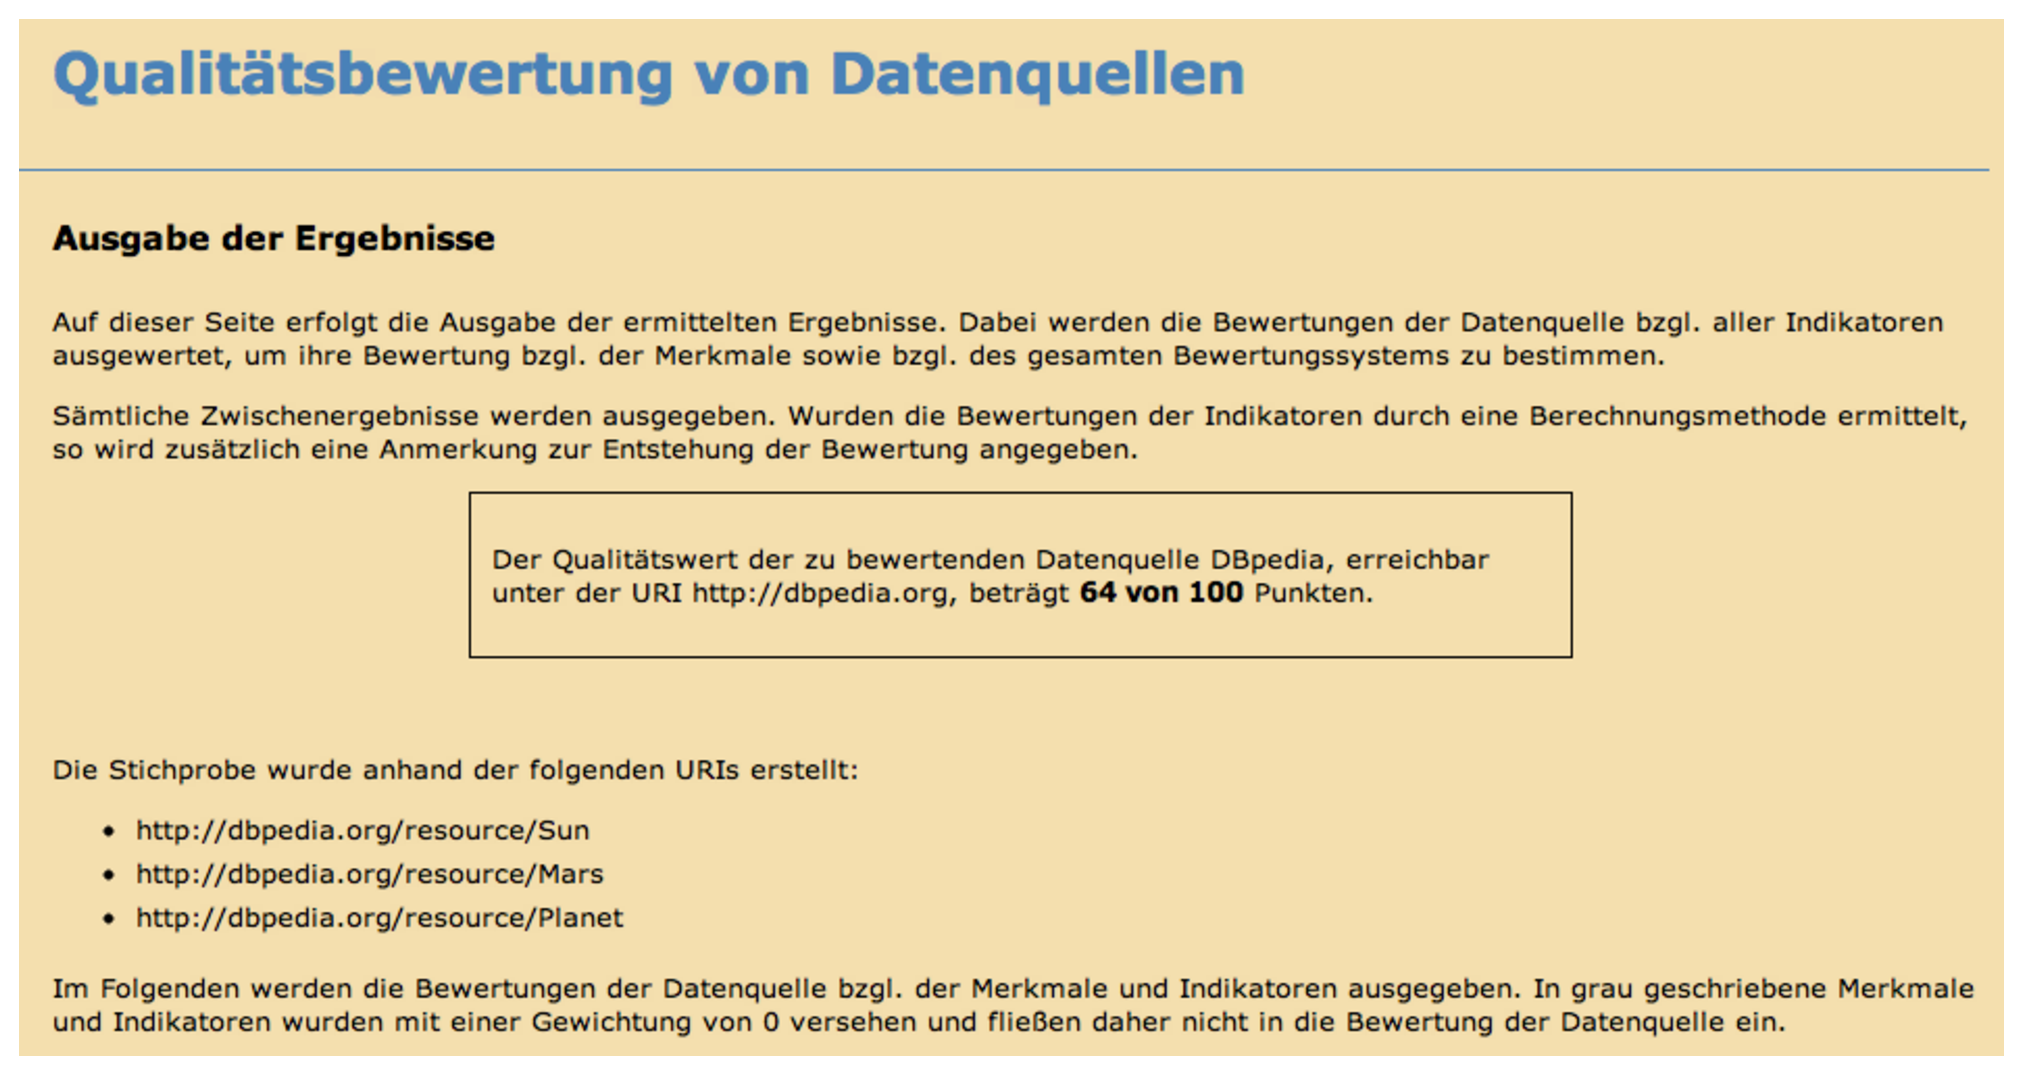
\includegraphics[width=3.5in]{Flemmingtool.pdf}
\caption{Excerpt of the Flemmings Data Quality Assessment tool showing the result of assessing the quality of DBpedia with a score of 64 out of 100.}
\label{fig:flemmingtool}
\end{figure}

On the one hand, the tool is easy to use with the form-based questions and adequate explanation for each step. 
Also, the assigning of the weights for each metric and the calculation of the score is straightforward and easy to adjust for each of the metrics. 
However, on the other hand, this tool has a few drawbacks: (1) the user needs to have adequate knowledge about the dataset in order to correctly assign weights for each of the metrics; (2) it does not drill down to the root cause of the proposed data quality problem and (3) some of the main quality dimensions are missing from the analysis such as accuracy, completeness, provenance, consistency, conciseness and relevancy as some could not be quantified and were not perceived to be true quality indicators. 

\paragraph{Sieve.}

\paragraph{LODGRefine.}
LODGRefine\footnote{\url{http://code.zemanta.com/sparkica/}} is a LOD-enabled version of Google Refine, which is an open source tool for working with messy data. 
Although this tool is not focused towards data quality assessment per-say, it is very powerful in performing preliminary cleaning or refining of raw data. 

Using this tool, one is able to import several different file types of data (CSV, Excel, XML, RDF/XML, N-Triples or even JSON) and then perform cleaning over it. 
In particular, it helps in detecting duplicates, discovering patterns (e.g. alternative forms of abbreviations), spotting inconsistencies (e.g. trailing white spaces), finding blank cells and similar errors. 

Additionally, this tool allows users to reconcile data, that is to connect a dataset to existing vocabularies such that it gives meaning to the field values. 
This feature thus assists in assessing as well as improving the data quality, in particular the interpretability, of a dataset. 
Reconciliations to Freebase\footnote{\url{http://www.freebase.com/}} helps mapping ambiguous textual values to precisely identified Freebase entities. 
Reconciling using Sindice or based on standard SPARQL or SPARQL with full-text search is also possible\footnote{\url{http://refine.deri.ie/reconciliationDocs}}.
Moreover, it is also possible to extend the reconciled data with DBpedia as well as exporting the data as RDF using this tool, which adds to the uniformity of the dataset.

LODGRefine is easy to download and install as well as to upload and perform basic cleansing steps on raw data.
The features of reconciliation, extending the data with DBpedia, exporting the data as RDF add to the usability, interpretability and uniformity of the dataset.
However, this tool has a few drawbacks: (1) the user is not able to perform detailed high level data quality analysis utilizing the various quality dimensions using this tool; (2) performing cleansing over a large dataset is time consuming as the tool follows a column data model and thus the user must perform transformations per column.
%Figure
%Drawback
 
\subsection{Summary and comparison of selected approaches}
%No, of papers from each year or each conference/journal - quantitative analysis

\section{Proposed Linked Data quality assessment steps}
% Which papers follow which steps
% Introduce the tools mentioned in Step 4
%Lay-users, tech users and domain experts
%
%A data quality assessment methodology is defined as the process of evaluation if a piece of data meets in the information consumers need in a specific use case~\cite{Bizer}.
%The process involves measuring the quality dimensions that are relevant to the user and comparing the assessment results with the users quality requirements.
%
%The steps of the assessment phase are:
%\begin{itemize}
%\item data analysis, which examines data schemas and performs interviews to reach a
%complete understanding of data and related architectural and management rules;
%\item DQ requirements analysis, which surveys the opinion of data users and administrators
%to identify quality issues and set new quality targets;
%\item identification of critical areas, which selects the most relevant databases and data
%flows to be assessed quantitatively;
%\item process modeling, which provides a model of the processes producing or updating
%data;
%\item measurement of quality, which selects the quality dimensions affected by the quality
%issues identified in the DQ requirements analysis step and defines corresponding
%metrics; measurement can be objective when it is based on quantitative metrics, or
%subjective, when it is based on qualitative evaluations by data administrators and
%users.
%\end{itemize}
%Note that in all the steps of the assessment phase, a relevant role is played by metadata
%that store complementary information on data for a variety of purposes, including
%data quality. Metadata often provide the information necessary to understand data
%and/or evaluate them.

As defined in Section~\ref{concepts}, a data quality assessment methodology is defined as the process of evaluation if a piece of data meets in the information consumers need in a specific use case~\cite{Bizer}.
In each of the identified approaches, we extracted the methodology that they followed to assess the quality of a dataset. 
Based on our analysis of the existing approaches as well as the evaluated tools, we identified a series of steps followed by majority of the approaches. 
We then adapted and revised the steps to align them with the data quality assessment process performed particularly for LOD as follows: 
\begin{enumerate}
\item Requirements analysis (optional)
\item Data Quality Checklist
\item Statistics and low-level analysis
\item Aggregated and higher level metrics
\item Comparison (optional)
\item Interpretation
\end{enumerate}

Table~\ref{metricsteps} comprises of the steps involved in the data quality assessment process. 
We also provide the input and output for each step along with a list of tools that would support at each step. 
Moreover, we identify the user involvement for each of the steps, that is, we identify whether the tool is automated, semi-automated or manual.
%The "Assessment steps" measures the quality of data collections along relevant quality dimensions; in particular the measurement of quality dimensions is provided by a set of metrics defined for each dimension. 

We now describe each of the steps in detail. 
\paragraph{\textbf{Requirements analysis (optional).}}
The multidimensionality of the information quality makes it dependent on a number of factors that can be achieved by the analyses of the user requirements. 
Thus, the use case in question is highly important when assessing the quality of a dataset.
This step is optional since it is not always provided in LOD related approaches and not all users necessarily have a use case in mind when assessing the quality of the dataset.
In other words, a user might just want to find out the completeness of a dataset and will not have any particular use case for that particular dataset.

\emph{Input.} As the input is the use case specified by the user with the aim of assessing the data quality of a particular dataset.

In this step, we identify two types of users: (a) those who know the problem with their dataset and (b) those who don't. 
Both users, however, are interested in finding the \emph{fitness of use} for their dataset.

\paragraph{\textbf{Data Quality Checklist.}}
After specifying a use case or after deciding to assess the quality of a dataset, the user then is presented with a list of data quality dimensions but only those that do not have a specified statistical metric available. 
That is those dimensions which can perhaps be measured qualitatively. 

\emph{Input.} In this step, a checklist of data quality dimensions are presented to the user, but only those dimensions which call upon a boolean answer. 
That is, the user has to either tick which dimensions are present or provide a 0 (no) if it not present or 1(yes) if it is present.

\emph{Output.} The output of this step is the result of the evaluation of these boolean dimensions, that is, a sum of 0's(no) or 1's(yes) which add to the final data quality assessment report. 

\emph{Tool Support.} Flemmings Data Quality Assessment tool\footnote{\url{http://linkeddata.informatik.hu-berlin.de/LDSrcAss/}} includes such questions in the process of data quality assessment.
For example, questions such as whether the datasets provides a message board or a mailing list pointing to the Comprehensibility dimension are asked to the user. 
Thus, the user involvement is entirely manual where the user must have knowledge about the details of the dataset to answer these questions.

\paragraph{\textbf{Statistics and low-level analysis.}}
This step performs basic statistical and low-level analysis on the dataset.
Generic statistics on the dataset are calculated. 

\emph{Input.} The input for this step is the dataset itself. 

\emph{Output.} The output is a statistical overview of the dataset. 
That is, it provides generic statistics on the dataset based on certain pre-defined heuristics.

\emph{Tool Support.} LODStats\footnote{\url{http://stats.lod2.eu/}} and LODGRefine\footnote{\url{http://code.zemanta.com/sparkica/}} are two tools identified to provide such basic analysis on a dataset.
LODStats gathers comprehensive statistics about a dataset available as RDF. 
It helps to know the structure, coverage and coherence of the data. 
It provides 32 different statistics such as property usage, vocabulary usage, datatypes used, average length of string literals, number of interlinks, to name a few. 
Thus, it helps to provide important insights with regard to the expected quality.
%screenshot?

LODGRefine, on the other hand, helps users import their dataset and presents them an overview of the possible short-comings of the dataset. 
For example, characteristics such as Completeness,  Interpretability of the column headers or Consistency is evident to the user. 
Moreover, it allows easy data cleansing mechanisms by performing transformations on a large amount of data at once. 
Additionally, LODGRefine also provides the functionality of reconciling data with Freebase\footnote{\url{http://www.freebase.com/}} or DBpedia, thus increasing the Coherency of the dataset.
Both these tools work automatically once a user uploads their dataset.

\paragraph{\textbf{Aggregated and higher level metrics.}} 
In this step, 

\emph{Input.} This step includes all the dimensions that are not included in the Data Quality Checklist step, that is those dimensions which can be measured quantitatively.   

\emph{Output.} 
As an output, a single metric or a combination of them produces a value within the range [0;1]. 

\emph{Tool Support.} 
There are a number of tools we identified that perform the tasks involved in this step. 
WIQA~\cite{Bizer} is a information quality assessment framework which allows users to apply a wide range of policies to filter information. 
When a user browses the web, WIQA runs in the background and analyses the web pages. 
It then extracts structured information from the page such as the quality-related as well as basic provenance information and stores it in a local repository. 
This stored information can then be filtered using quality-based information filtering policies to show only information matching the policy. 
These policies take into account the different types of quality-related meta-information available in the dataset. 
It is a semi-automated tool that can help to perform 

ProLOD~\cite{Bohm} is another tool that works semi-automatically  in which the triples of a dataset is stored in a relational database. 
The triples are then enriched with data type and pattern information and are divided into clusters.
Then the user can select a particular cluster, the facts and statistics of which is presented in detail. 
The tool helps in discovering poor attributes (i.e. those that do not contain useful values for most data entries), occurrence dependencies (e.g. book entity from a media cluster), negative dependencies (e.g. negative associations between the predicates author and developer in a media closer) as well as misusage among predicates.

Flemmings Data Quality Assessment Tool~\cite{Flemming} also supports in calculating higher level metrics 
%Ex: WIQA, ProLOD, Flemming, LinkQA, W3C's RDF Validator + other validators, Sieve, EvoPat, ORE


\paragraph{\textbf{Comparison (optional).}}
Used when the resulted measurements provided in step "Aggregated and higher level metrics" are compared to reference values such as previous values from dataset in the same domain or gold standard values, in order to enable a diagnosis of quality. 

\emph{Input.} 
"Target/derived dataset (eg. Geonames)
Assessment results from step 2 and 4
Original dataset (eg. OpenStreetMap)"

\emph{Output.} 
evaluation of the representation
evaluation between datasets in the same domain"

\emph{Tool Support.} 
%Not come across any tools, highly domain dependant

\paragraph{\textbf{Interpretation.}}
Gives an interpretation to the results obtained from step Data Quality Checklist.

\emph{Input.} 
Assessment results from Step 2 and 4

\emph{Output.} 
Explanation of the results

\emph{Tool Support.} 
%Ex in WIQA

\begin{table*}[htb]
\caption{Data quality assessment steps}
\label{metricsteps}
\begin{tabular}{ | p{2cm} | p{3.3cm} | p{3.7cm} | p{1.5cm} | c | c | c | }
\hline
\textbf{Steps} & \textbf{Input} & \textbf{Output} & \textbf{Tool support} & \multicolumn{2}{c}{\textbf{User involvement }} & \cr
\hline
& & & & \textbf{Automated} & \textbf{Semi-automated} & \textbf{Manual} \\
\hline
\textbf{Requirements analysis (optional)} & Assessment of data quality, 2 types of users: \begin{itemize} \item who know the problem with their dataset \item who do not know the problem with their dataset \end{itemize} & - & - & - & - & - \\
\hline
\textbf{Data quality checklist} & Checklist of dimensions which have a binary evaluation & Results of the evaluation - 0 (no) or 1 (yes) & Flemming et al., 2010  & - & - & - \\
\hline
\textbf{Statistics and low level analysis} & Dataset & \multirow{3}{*}{Overview statistics of the dataset} & LODStats & \tick & - & - \\
\cline{4-7}
 & & & LODGRefine & \tick & - & - \\
\hline
\textbf{Aggregated and higher level metrics} & Dimensions not included in Step 2 & \multirow{8}{3cm}{Results of the evaluation of these dimensions in a range from 0 to 1}
 & WIQA & - & \tick & -  \\
 \cline{4-7}
 & & & ProLOD & - & \tick & - \\
 \cline{4-7}
 & & & Flemming et al., 2010 & - & \tick & - \\
 \cline{4-7}
 & & & LinkQA & \tick & - & - \\
 \cline{4-7}
 & & & W3C's RDF Validator & - & \tick & - \\
 \cline{4-7}
 & & & Sieve & - & - & \tick \\
 \cline{4-7}
 & & & EvoPat & - & - & \tick \\
 \cline{4-7}
 & & & ORE & - & \tick & - \\
\hline
\textbf{Comparison (optional)} & \begin{itemize} \item Target/derived dataset \item Assessment results from step 2 and 4 \item Original dataset \end{itemize} & \begin{itemize} \item Evaluation of the representation \item Evaluation between datasets in the same domain \end{itemize} & - & - & - & - \\
\hline
\textbf{Interpretation} & Assessment results from Step 2 and 4 & Explanation of the results & WIQA & - & - & \tick \\
\hline
\end{tabular}
\end{table*}


%\section{Discussion}\label{sec:disc}
%\input{discussion}

\section{Conclusions and open issues }
\label{sec:conc}

%Only few approaches implemented a tool
%None covered all aspects of data quality (all dimensions)
% All approaches at their core describe....
%Level of automation - some were automated so user could not put in their own data. Others were manual which required a considerable amount of configuration and some others were semi-automated, which were although easy to use had a big pay off in the quality of the results
%Quality of the results varied among the approaches
%Formal definitions
%Metrics
%muddy these conceptual waters very quickly

%This limitation can be attributed to the infancy of this domain. As it is only over the past 3 years that there has been the production of machine readable data.

\subsection{Open issues}

%\begin{figure}[t]
%\leavevmode\fbox{\parbox[b][30mm][s]{30mm}{
%\vfill\footnotesize Please include graphics in Encapsulated
%PostScript (.eps) format\vfill}}
%\caption{Figure caption.}
%\end{figure}

%\begin{table*}[htb]
%\caption{Table caption} \label{t1}
%\begin{tabular}{ll d{1.3} d{1.3} d{1.3} d{1.3} d{1.3} d{1.3}}
%\hline
%Dataset&Models&\multicolumn{1}{l}{$\alpha_1$}&
%\multicolumn{1}{l}{$\alpha_2$}&
%\multicolumn{1}{l}{$\alpha_3$}&
%\multicolumn{1}{l}{$\alpha_4$}&
%\multicolumn{1}{l}{$\alpha_5$}&
%\multicolumn{1}{l}{$\alpha_6$}\\
%\hline
%CSDS&Linear     &0.164&0.22&0.123&0.3&0.200&0.258\\
%& Logistic      &0.189&0.155&0.157&0.201&0.154&0.144\\[6pt]
%KCDS&Linear     &0.155&0.183&0.160&0.218&0.176&0.156\\
%& Logistic      &0.187&0.125&0.151&0.184&0.187&0.125\\
%\hline
%\end{tabular}
%\end{table*}

\bibliographystyle{acm}
\bibliography{biblio}
%\begin{thebibliography}{0}

%\bibitem{1} L. Lamport, \textit{\LaTeX{} User's Guide \& Reference Manual}, Addison Wesley Publishing Co, 1985.

%\bibitem{2} B. Newman and E.T. Liu, Perspective on BRCA1, \textit{Breast Disease} \textbf{10} (1998), 3--10.

%\bibitem{3} D.F. Pilkey, \textit{Happy conservation laws}, in: Neural Stresses, J. Frost, ed., Controlled Press, Georgia, 1995, pp. 332--391.

%\bibitem{4} E. Wilson, \textit{Active vibration analysis of thin-walled beams}, Ph.D. Dissertation, University of Virginia, 1991.

%\end{thebibliography}

\end{document}
